\documentclass[10pt]{beamer}

\usetheme[navigation]{UMONS}
\usepackage[listings]{tcolorbox}
\usepackage{booktabs}

\usepackage[utf8]{inputenc}
\usepackage{verbatim}
\usepackage[T1]{fontenc}
\usepackage[utf8]{inputenc}
\usepackage{amsmath,bm}
\usepackage{amsfonts}
\usepackage{amssymb}
\usepackage{multirow}
\usepackage{multicol}

%\usepackage{utopia}
%\usepackage{charter}
%\usepackage{pifont}
%mathptmx, helvet, avat, bookman, 
%chancery, charter, culer, mathtime, 
%mathptm, newcent, palatino, pifont,
%utopia.
%\usefonttheme{professionalfonts} % using non standard fonts for beamer
%\usepackage{fontspec}
    %setting a font
%\setsansfont{Adobe Garamond Pro}

%\setmainfont{Adobe Garamond Pro}
%   
%\usefonttheme[stillsansseriflarge]{serif}
%\usefonttheme{default}


%\usepackage{tgbonum}
%\usepackage[left=1in, right=1in, top=0.5in, bottom=1in]{geometry}

\usepackage{listings}
\usepackage{color}
\usepackage{verbatim}
\usepackage{fancyvrb}
\usepackage{lhelp}
\usepackage{xcolor}
%\usepackage[table, svgnames, dvipsnames]{xcolor}

\usepackage{hyperref} %comment out for hardcopy
\hypersetup{
	colorlinks,
	linkcolor={blue!50!black},
    citecolor={blue!50!black},
    urlcolor={blue!80!black}
   }

\newif\ifcomment
\commentfalse


%\usepackage [english]{babel}
%\usepackage [autostyle, english = american]{csquotes}
%\MakeOuterQuote{"}

%\usepackage[T1]{fontenc}
%\usepackage{textcomp}
%\usepackage [english]{babel}
%\usepackage [autostyle, english = american]{csquotes}
%\MakeOuterQuote{"}

\usepackage{pgfplots}
\pgfplotsset{compat=1.13}
%%%%%%%%%%%%%%%%%%%%%%%%%%%%%%%%%%%%
\pgfkeys{
     /pgf/number format/precision=2, 
    /pgf/number format/fixed zerofill=true,
    /pgf/number format/fixed
}
%%%%%%%%%%%%%%%%%%%%%%%%%%%%%%%%%%%%

\usepackage{tikz}
\usetikzlibrary{patterns}
%\usetikzlibrary{shadows.blur}

%\usepackage{helvet}
%\usepackage{fontspec}

%\usepackage{xcolor}
%\newcommand\code{{\fontsize{8}{8}$\#$}\fontfamily=\ttfamily \fontsize{8}{8}\selectfont}
\newcommand\term{{\fontsize{8}{8}}\fontfamily=\ttfamily \fontsize{8}{8}\selectfont}

%\setlist[itemize]{noitemsep, topsep=0pt}
%%\setlist[itemize]{itemsep=0.05pt, topsep=0pt}
%\setlist[enumerate]{noitemsep, topsep=0pt}
%\setlist[enumerate]{itemsep=0.2pt, topsep=0pt}

\let\oldcenter\center
\let\oldendcenter\endcenter
\renewenvironment{center}{\setlength\topsep{0pt}\oldcenter}{\oldendcenter}

%\renewcommand{\baselinestretch}{1.2}
\setlength{\parindent}{0pt}
\setlength{\parskip}{1.3ex}
\usepackage[nodisplayskipstretch]{setspace}
%\setstretch{1.4}
\setlength{\leftmargini}{8pt}
%\addtobeamertemplate{block begin}{%
%  \setlength{\textwidth}{1.2\textwidth}%
%}{}


\setlength{\textfloatsep}{0.075em}% Remove \textfloatsep
\setlength{\floatsep}{0.025ex}% Remove \textfloatsep
\setlength{\intextsep}{0.025em}% Remove \textfloatsep


\setlength{\belowcaptionskip}{0.5em}

\usepackage{algorithm}
%\usepackage[ruled,vlined,linesnumbered]{algorithm2e}
%\usepackage{algorithmicx}
\usepackage{algcompatible}
\usepackage{algpseudocode}

\algrenewcommand\algorithmicend{\textsf{\textbf{end}}}
\algrenewcommand\algorithmicdo{\textsf{\textbf{do}}}
\algrenewcommand\algorithmicwhile{\textsf{\textbf{while}}}
\algrenewcommand\algorithmicfor{\textsf{\textbf{for}}}
\algrenewcommand\algorithmicforall{\textsf{\textbf{for all}}}
\algrenewcommand\algorithmicloop{\textsf{\textbf{loop}}}
\algrenewcommand\algorithmicrepeat{\textsf{\textbf{repeat}}}
\algrenewcommand\algorithmicuntil{\textsf{\textbf{until}}}
\algrenewcommand\algorithmicprocedure{\textsf{\textbf{procedure}}}
\algrenewcommand\algorithmicfunction{\textsf{\textbf{function}}}
\algrenewcommand\algorithmicif{\textsf{\textbf{if}}}
\algrenewcommand\algorithmicthen{\textsf{\textbf{then}}}
\algrenewcommand\algorithmicelse{\textsf{\textbf{else}}}
\algrenewcommand\algorithmicrequire{\textsf{\textbf{Require:}}}
\algrenewcommand\algorithmicensure{\textsf{\textbf{Ensure:}}}
\algrenewcommand\algorithmicreturn{\textsf{\textbf{return}}}

\usepackage{caption}

% primary blue 33 7a b7
% info blue 31 70 8f

%\definecolor{wp}{rgb}{0.29,0.14,0.47}
%\definecolor{wpbright}{rgb}{0.58,0.45,0.74}

\definecolor{wp}{rgb}{0.129,0.478, 0.678}
%\definecolor{wp}{rgb}{0.26,0.55, 0.79}
%\definecolor{wpbright}{rgb}{0.192, 0.439, 0.561}\\
%\definecolor{wpbright}{rgb}{0.43, 0.43, 0.43}
%\definecolor{wp}{rgb}{0.19, 0.45, 0.66}
\definecolor{wpbright}{rgb}{0.26,0.55, 0.79}

\definecolor{yellowBright}{HTML}{FFD247}
\definecolor{orangeBright}{HTML}{FF7E47}
\definecolor{gray1}{HTML}{CEDBE1}
\definecolor{gray2}{HTML}{DDE6EA}
\definecolor{gray3}{HTML}{E3E6EB}
\definecolor{darkblue1}{HTML}{2375B9}%{0A599B}
\definecolor{darkblue2}{HTML}{3D577A}
\definecolor{lightblue1}{HTML}{65A4D9}
\definecolor{lightblue2}{HTML}{94C3E9}
\definecolor{red1}{HTML}{E4001B}
\definecolor{red2}{HTML}{8F2831}
\definecolor{lime1}{HTML}{AEBD63}
\definecolor{navy}{HTML}{000063}
\definecolor{pistachio}{HTML}{99CC66}
\definecolor{burgundy}{HTML}{900020}
\definecolor{coolgrey}{HTML}{8c92ac}
\definecolor{green1}{HTML}{A4C639}
\definecolor{byzantium}{HTML}{702963}
\definecolor{pastelgreen}{HTML}{03c03c}

\definecolor{purple1}{HTML}{8F2831}
\definecolor{contrast}{HTML}{CE0000}
%\colorlet{mycolor}{someothercolor}

\definecolor{positive}{HTML}{0D900F}
\definecolor{negative}{HTML}{FF0000}

\definecolor{dNone}{HTML}{FFFFFF}
%\definecolor{dOne}{HTML}{yellow}
%\definecolor{dTwo}{HTML}{blue}
%\definecolor{dThree}{HTML}{green}
%\definecolor{dFour}{HTML}{red}
\colorlet{dOne}{coolgrey!70}
\colorlet{dTwo}{pistachio!70}
\colorlet{dThree}{lightblue1!70}
\colorlet{dFour}{negative!70}

\colorlet{dOneLight}{dOne!40}
\colorlet{dTwoLight}{dTwo!40}
\colorlet{dThreeLight}{dThree!40}
\colorlet{dFourLight}{dFour!40}




%%%%%%%%%%%%%%%%%%%%%%%%%%%%%%%%%%%%%%%%%%%%%%%%%%
%\newcommand{\zpz}{$\mathbb{Z}/p\mathbb{Z}$}
%\newcommand{\mz}{$\mathbb{Z}$}
%\newcommand{\Z}{\mathbb{Z}}
%\newcommand{\Q}{\mathbb{Q}}
%\newcommand{\local}{\texttt{{\bf local: }}}
%\newcommand{\tid}{\local {\texttt{tid := blockIdx.x$*$blockSize.x$+$threadIdx.x}}}
%\newcommand{\mword}{of a machine-word}
%\newcommand{\initzero}{all digits initially set to 0}
%\newcommand{\algskeleton}{Template}
%\newcommand{\changeToAlgSkeleton}{
%\renewcommand{\thealgorithm}{}
%%	\renewcommand{\thealgorithm}{}
%	\renewcommand{\addcontentsline}[3]{}
%	\floatname{algorithm}{\algskeleton}
%	}
%\newcommand{\twiddle}[2]{D_{K,{#1}}}
%\def\DFT{\ensuremath{\mathrm{DFT}}}
%\newcommand{\cumodp}{CUMODP}
%
%\def\DFT{\ensuremath{\mathrm{DFT}}}
%\def\xx{\ensuremath{\mathbf{x}}}
%\def\yy{\ensuremath{\mathbf{y}}}
%%%%%%%%%%%%%%%%%%%%%%%%%%%%%%%%%%%%%%%%%%%%%%%%%%



%\newcolumntype{redcolor}{>{\columncolor{red}}c}

\usepackage{cmap}
\usepackage{bibentry}
\usepackage{listings}
\usepackage{slantsc}
\usepackage{array}
\captionsetup{compatibility=false}
\usepackage{minted}
\usetikzlibrary{arrows.meta}
\usetikzlibrary{chains}
\usepackage{algorithm}
%\usepackage[ruled,vlined,linesnumbered]{algorithm2e}
%\usepackage{algorithmic}
\usepackage{algcompatible}
\usepackage{algpseudocode}

\usepackage{graphicx}
\usepackage{float}
\usepackage{subcaption}
\usepackage{ulem}

\usepackage{animate}
\usepackage{media9}
\usetikzlibrary{patterns}
\tikzset{every path/.style=thick}
\usepackage{pgfplots}
\usepgfplotslibrary{polar}
\usepgflibrary{shapes.geometric}
\usetikzlibrary{calc}
\pgfplotsset{my style/.append style={axis x line=middle, axis y line=
		middle, xlabel={$x$}, ylabel={$y$}, axis equal }}

\usepackage{xcolor}
\expandafter\def\expandafter\normalsize\expandafter{%
	\normalsize
	\setlength\abovedisplayskip{0pt}
	\setlength\belowdisplayskip{0pt}
	\setlength\abovedisplayshortskip{0pt}
	\setlength\belowdisplayshortskip{0pt}
}
%%%%%%%%%%%%%%%%%%%%%%%%%%
%%%% Mathematical Sets %%%
%%%%%%%%%%%%%%%%%%%%%%%%%%
%% \def\A{\mbox{${\mathbb A}$}}
\def\B{\mbox{${\mathbb B}$}}
\def\C{\mbox{${\mathbb C}$}}
\def\F{\mbox{${\mathbb F}$}}
%\def\H{\mbox{${\mathbb H}$}}
\def\K{\mbox{${\mathbb K}$}}
\def\N{\mbox{${\mathbb N}$}}
\def\Q{\mbox{${\mathbb Q}$}}
\def\R{\mbox{${\mathbb R}$}}
\def\Z{\mbox{${\mathbb Z}$}}

%%%%%%%%%%%%%%%%%%%%
%% Linear algebra %%
%%%%%%%%%%%%%%%%%%%%
\def\A {\ensuremath{\mathbf{A}}}
\def\BB {\ensuremath{\mathbf{B}}}
\def\CC {\ensuremath{\mathbf{C}}}
\def\D {\ensuremath{\mathbf{D}}}
\def\E {\ensuremath{\mathbf{E}}}
\def\G {\ensuremath{\mathbf{G}}}
\def\H {\ensuremath{\mathbf{H}}}
\def\M {\ensuremath{\mathbf{M}}}
\def\NN {\ensuremath{\mathbf{N}}}
\def\P {\ensuremath{\mathbf{P}}}
\def\QQ {\ensuremath{\mathbf{Q}}}
\def\S {\ensuremath{\mathbf{S}}}
\def\U {\ensuremath{\mathbf{U}}}
\def\V {\ensuremath{\mathbf{V}}}
\def\a {\ensuremath{\mathbf{a}}}
\def\b {\ensuremath{\vec{b}}}
\def\c {\ensuremath{\mathbf{c}}}
\def\d {\ensuremath{\mathbf{d}}}

\def\i {\ensuremath{\mathbf{i}}}
\def\j {\ensuremath{\mathbf{j}}}
\def\k {\ensuremath{\mathbf{k}}}
\def\m {\ensuremath{\mathbf{m}}}
\def\n {\ensuremath{\mathbf{n}}}
\def\p {\ensuremath{\mathbf{p}}}

\def\q {\ensuremath{\mathbf{q}}}
\def\t {\ensuremath{\mathbf{t}}}
\def\x {\ensuremath{\vec{x}}}
\def\u {\ensuremath{\mathbf{u}}}
\def\v {\ensuremath{\mathbf{v}}}
\def\w {\ensuremath{\mathbf{w}}}
\def\y {\ensuremath{\mathbf{y}}}
\def\z {\ensuremath{\mathbf{z}}}
\def\e {\ensuremath{\vec{e}}}
\def\0 {\ensuremath{\mathbf{0}}}
\newcommand{\Zero}[1]{\ensuremath{{\mathbf{0}}^{#1}}}
\newcommand{\rank}[1]{\ensuremath{{\rm rank}(#1)}}
\newcommand{\norm}[1]{\ensuremath{ \| {#1} \| }}



%%%%%%%%%%%%%%%%%%%%%%%%%%%%%%%%
%%% Computer algebra systems %%%
%%%%%%%%%%%%%%%%%%%%%%%%%%%%%%%%
\newcommand{\axiom}{\mbox{{\sc Axiom}}}
\newcommand{\axiomxl}{\mbox{{\sc AXIOM-XL}}}
\newcommand{\aldor}{\mbox{{\sc Aldor}}}
\newcommand{\gb}{\mbox{{\sc GB}}}
\newcommand{\basicmath}{\mbox{{\em BasicMath}}}
\newcommand{\aldorlib}{\mbox{{\em aldorlib}}}
\newcommand{\algebralib}{\mbox{{\em libalgbra}}}
\newcommand{\magma}{{\sc Magma}}
\newcommand{\maple}{{\sc Maple}}
\newcommand{\Maple}{{\sc Maple}}
\newcommand{\mathematica}{{\sc Mathematica}}
\newcommand{\matlab}{{\sc Matlab}}
\newcommand{\java}{{\sc Java}}
\newcommand{\pascal}{{\sc Pascal}}
\newcommand{\reduce}{{\sc Reduce}}
\newcommand{\singular}{{\sc Singular}}
\newcommand{\ntl}{\mbox{{\sc NTL}}}

%\def\language#1{\texttt{#1}}
\def\package#1{\textsc{#1}}
%\def\function#1{\textrm{#1}}
\def\userfunction#1{\textsf{#1}}
%\def\algorithm#1{\textsc{#1}}
\def\mathsymbol#1{\mbox{$#1$}}
%%\def\maple{\mbox{{\sc Maple}}}
%%\def\axiom{\mbox{{\sc AXIOM}}}
%%\def\aldor{\mbox{{\sc Aldor}}}
\def\fortran{\mbox{{\sc FORTRAN}}}
\def\scratchpad{{\tt scratchpad}}
%%\def\singular{\mbox{{\sc Singular}}}
\def\diffAlg{\mbox{{\sc DiffAlg}}}
\def\triade{\mbox{{\sc triade}}}
\def\kronecker{\mbox{{\tt Kronecker}}}
%% \def\delta{\mbox{{$\Delta$}}}
\def\Piit{\mbox{{${\Pi}^{it}$}}}
\def\sumit{\mbox{{${\Sigma}^{it}$}}}
\def\libaldor{\mbox{{\sc libaldor}}}
\def\libalgebra{\mbox{{\sc libalgebra}}}
\def\pardi{\mbox{{\sf Pardi}}}
\def\riff{\mbox{{\tt Riff}}}
\def\modpone{\mbox{{\tt modp1}}}
\def\modptwo{\mbox{{\tt modp2}}}
\def\recden{\mbox{{\tt recden}}}
\def\algebraic{\mbox{{\tt algebraic}}}

\def\RegularChains{\mbox{{\tt RegularChains}}}
\def\modpn{\mbox{{\tt modpn}}}
\def\cumodp{\mbox{{\tt CUMODP}}}
\def\bpas{\mbox{{\tt BPAS}}}
\def\ProgramAnalysis{\mbox{{\tt ProgramAnalysis}}}

\def\spiral{\mbox{\sc SPIRAL}}
\def\kaapi{\mbox{\sc Kaapi}}
\def\fasttriade{\mbox{\sc FastTriade}}
\def\cogepas{\mbox{\sc CoGePas}}
\def\pascolib{\mbox{{\sc PASCOLib}}}
\def\hpcsolve{\mbox{\sc HpcSolve}}
\def\cadyna{\mbox{\sc CADYNA}}

\newcommand{\cilk}{\mbox{\sc Cilk}}
\newcommand{\cilkview}{\mbox{\sc Cilkview}}
\newcommand{\cilkplus}{\mbox{\sc Cilkplus}}
\newcommand{\cilkp}{\mbox{\sc Cilk-P}}
\newcommand{\nvcc}{\mbox{\sc nvcc}}
\newcommand{\openmp}{\mbox{\sc OpenMP}}
\newcommand{\openmptasks}{\mbox{\sc OpenMP Tasks}}
\newcommand{\meta}{\mbox{\sc MetaFork}}
\newcommand{\ppcg}{\mbox{\sc PPCG}}
\newcommand{\ctocuda}{\mbox{\sc C-to-CUDA}}
\newcommand{\hicuda}{\mbox{\sc HiCUDA}}
\newcommand{\cudachill}{\mbox{\sc CUDA-CHiLL}}
\newcommand{\clang}{\mbox{\sc Clang}}
\newcommand{\llvm}{\mbox{\sc LLVM}}
\newcommand{\ptx}{\mbox{\sc PTX}}
\newcommand{\nvptx}{\mbox{\sc NVPTX}}
\newcommand{\tbb}{\mbox{\sc TBB}}
\newcommand{\openacc}{\mbox{\sc OpenACC}}
\newcommand{\opencl}{\mbox{\sc OpenCL}}
\newcommand{\cplusplusamp}{\mbox{\sc C++ AMP}}
\newcommand{\cuda}{\mbox{\sc CUDA}}
\newcommand{\gpu}{\mbox{\sc GPU}}
\newcommand{\ibmxl}{\mbox{\sc IBM XL}}


%% \bibliographystyle{abbrv} %% OK !!
%% \bibliographystyle{plain}
%% \bibliographystyle{apalike} %% KO 
%%\bibliographystyle{ieeetr} %% OK !
%% \bibliographystyle{siam}  %% KO 
%% \bibliographystyle{unsrt} %% OK !
%% \bibliographystyle{alpha}
%% \leftmargini=20pt

%%%%%%%%%%%%%%%%%%%%%%%%%
%%% Theorems and such %%%
%%%%%%%%%%%%%%%%%%%%%%%%%
%\newtheorem{corollary}{Corollary}
%\newtheorem{theorem}{Theorem}
%\newtheorem{lemma}{Lemma}
%\newtheorem{problem}{Problem}
%\newtheorem{definition}{Definition}
%\newtheorem{proposition}{Proposition}
%\newtheorem{notation}{Notation}
%\newtheorem{example}{Example}
%\newtheorem{hypothesis}{Hypothesis}
%\newtheorem{remark}{Remark}

%\algnewcommand\algorithmicswitch{\textbf{switch}}
%\algnewcommand\algorithmiccase{\textbf{case}}
%\algnewcommand\algorithmicassert{\texttt{assert}}
%\algnewcommand\Assert[1]{\State \algorithmicassert(#1)}%
% New "environments"
%\algdef{SE}[SWITCH]{Switch}{EndSwitch}[1]{\algorithmicswitch\ #1\ \algorithmicdo}{\algorithmicend\ \algorithmicswitch}%
%\algdef{SE}[CASE]{Case}{EndCase}[1]{\algorithmiccase\ #1}{\algorithmicend\ \algorithmiccase}%
%\algtext*{EndSwitch}%
%\algtext*{EndCase}%

%\newenvironment{Proof}{ {\noindent} {\sc Proof} $\rhd$}{$\lhd$}

%%%%%%%%%%%%%%%%%%%%%%%%%%%%%
%% Operations on polyhedra %%
%%%%%%%%%%%%%%%%%%%%%%%%%%%%%
\newcommand{\can}[1]{\mbox{{\sf can}$(#1)$}}
\newcommand{\proj}[1]{\mbox{{\sf proj}$(#1)$}}
\newcommand{\dproj}[1]{\mbox{{\sf Dproj}$(#1)$}}
\newcommand{\gproj}[1]{\mbox{{\sf Gproj}$(#1)$}}
\newcommand{\sol}[1]{\mbox{$V_{\Z}(#1)$}}

\newcommand{\isolve}[1]{\mbox{{\sf IntegerSolve}$(#1)$}}
\newcommand{\LP}[1]{\mbox{{\sf LP}$(#1)$}}



%%%%%%%%%%%%%%%%%%%%%%%%%%%%
%%% Miscellaneous macros %%%
%%%%%%%%%%%%%%%%%%%%%%%%%%%%
\newcommand{\hidetext}[1]{\mbox{ \ }}
\newcommand{\todo}[2]{{{\textcolor{red}{ #1}}}\footnote{ {\textcolor{blue}{ #2}} }}
\newcommand{\todolater}[2]{#1}
\newcommand{\fix}[3]{#1}
%% \newcommand{\reworked}[1]{{{\textcolor{blue}{ #1}}}}
\newcommand{\reworked}[1]{{ #1}}
\newcommand{\newfixed}[1]{{\color{black} #1}}

%%%%%%%%%%%%%%%%%%%%%%%%%%%%%%%%
%%% Computer algebra systems %%%
%%%%%%%%%%%%%%%%%%%%%%%%%%%%%%%%
\newcommand{\altran}{{\sc ALTRAN}}
\newcommand{\trip}{{\sc Trip}}
\newcommand{\pari}{{\sc Pari}}
\newcommand{\flint}{\mbox{{\sc FLINT}}}
\newcommand{\sympy}{\mbox{{\sc SymPy}}}
\newcommand{\cocoa}{\mbox{{\sc CoCoA}}}
\newcommand{\cocoalib}{\mbox{{\sc CoCoALib}}}
\newcommand{\symboliccpp}{\mbox{{\sc SymbolicC++}}}
\newcommand{\mmx}{\mbox{{\sc Mathemagix}}}
\newcommand{\linbox}{\mbox{{\sc LinBox}}}
\newcommand{\sage}{\mbox{{\sc SageMath}}}

\newcommand{\myproof}{\textsc{Proof.} }
\newcommand{\myfoorp}{\hfill$\square$}

\newcommand{\euclideanDivision}[4]{\mbox{{$ \begin{array}{c|c} #1 & #2 \\ \cline{2-2}
				#3 & #4 \\ \end{array} $}}}
%\newtheorem{Hypothesis}{Hypothesis}
%\newtheorem{Algorithm}{Algorithm}
%\newtheorem{theorem}{Theorem}
%\newtheorem{Lemma}{Lemma}
%\newtheorem{Corollary}{Corollary}
%\newtheorem{Conjecture}{Conjecture}
%\newtheorem{Proposition}{Proposition}
%\newtheorem{Definition}{Definition}
%\newtheorem{Notation}{Notation}
%\newtheorem{Example}{Example}
%\newtheorem{Remark}{Remark}
%\newtheorem{Problem}{Problem}
%\newtheorem{Acknowledgment}[]{Acknowledgment}
%\iffalse
%\newenvironment{proof}{\noindent{\em Proof:}}{$\Box$~\\}
%\fi
%%%%%%%%%%%%%%%%%%%%%%%%%%%%%%%%%%%%%%%%%%%%%
%% Math Symbol Macros
%%%%%%%%%%%%%%%%%%%%%%%%%%%%%%%%%%%%%%%%%%%%%
\def\B {\ensuremath{\mathbb{B}}}
%\def\A {\ensuremath{\mathbb{A}}}
\def\C {\ensuremath{\mathbb{C}}}
\def\I {\ensuremath{\mathcal{I}}}
\def\J {\ensuremath{\mathcal{J}}}
\def\K {\ensuremath{\mathbb{K}}}
\def\L {\ensuremath{\mathbb{L}}}
\def\N {\ensuremath{\mathbb{N}}}
\def\V {\ensuremath{\mathcal{V}}}
\def\W {\ensuremath{\mathcal{W}}}
\def\Q {\ensuremath{\mathbb{Q}}}
\def\R {\ensuremath{\mathbb{R}}}
\def\Z {\ensuremath{\mathbb{Z}}}
%\def\KK {\ensuremath{\overline{\mathbb{K}}}}

\newcommand{\T}{\mathfrak{T}}
%\newcommand{\G}{\mathcal{G}}
\renewcommand{\O}{\ensuremath{\mathcal{O}}}
\renewcommand{\o}{\ensuremath{\underline{o}}}

%%\def\u {\ensuremath{\mathbf{u}}}
%\def\U {\ensuremath{\underline{U}}}
\def\x {\ensuremath{\mathbf{x}}}
\def\X {\ensuremath{\underline{X}}}
\def\y {\ensuremath{\mathbf{y}}}
\def\Y {\ensuremath{\underline{Y}}}
\def\xx{\ensuremath{\underline{x}}}
\def\yy{\ensuremath{\underline{y}}}
\def\li{\ensuremath{\langle}}
\def\ri{\ensuremath{\rangle}}

%\newcommand{\NN}{\mbox{$N_{\geq}$}}
%\renewcommand{\PP}{\mbox{$P_{>}$}}
\newcommand{\HH}{\mbox{$H_{\neq}$}}
%\def\QQ {\ensuremath{\mathcal{Q}}}
\def\UU {\ensuremath{\mathcal{U}}}
%\def\VV {\ensuremath{\mathcal{V}}}

\newcommand{\limit}[1]{\mbox{${\lim}(#1)$}}

\renewcommand{\hat}[1]{\mbox{$\widehat{#1}$}}
\renewcommand{\tilde}[1]{\mbox{$ \overset{\thicksim}{#1} $}}



%%%%%%%%%%%%%%%%%%%%%%%%%%%%%%%%%%%%%%%%%%%%%
%% Polynomials and regular chains
%%%%%%%%%%%%%%%%%%%%%%%%%%%%%%%%%%%%%%%%%%%%%
\newcommand{\discrim}[1]{\mbox{{\rm discrim}$(#1)$}}
\newcommand{\init}[1]{\mbox{{\rm init}$(#1)$}}
\newcommand{\iter}[1]{\mbox{{\rm iter}$(#1)$}}
\newcommand{\mdeg}[1]{\mbox{{\rm mdeg}$(#1)$}}
\newcommand{\mvar}[1]{\mbox{{\rm mvar}$(#1)$}}
\newcommand{\prem}[1]{\mbox{{\rm prem}$(#1)$}}
\newcommand{\pquo}[1]{\mbox{{\rm pquo}$(#1)$}}
%\newcommand{\rank}[1]{\mbox{{\rm rank}$(#1)$}}
\newcommand{\ires}[1]{\mbox{{\rm ires}$(#1)$}}
\newcommand{\OpenCAD}[1]{\mbox{{\sf OpenCAD}$(#1)$}}
\newcommand{\OpenAugCAD}[1]{\mbox{{\sf OpenCAD}$(#1)$}}
\newcommand{\LazyRealTriangularize}[1]{\mbox{{\sf LazyRealTriangularize}$(#1)$}}
\newcommand{\GenerateFormula}[1]{\mbox{{\sf GenerateFormula}$(#1)$}}
\newcommand{\RealRootCounting}[1]{\mbox{{\sf RealRootCounting}$(#1)$}}
\newcommand{\ReviseFormula}[1]{\mbox{{\sf Disjunction}$(#1)$}}
\newcommand{\SamplePoints}[1]{\mbox{{\sf SamplePoints}$(#1)$}}
\newcommand{\factor}[1]{\mbox{{\sf factor}$(#1)$}}
\newcommand{\ProjectionFactorSet}[1]{\mbox{{\sf ProjectionFactorSet}$(#1)$}}
\newcommand{\notdone}{{\tt NotDone}}
\newcommand{\Intersect}[1]{\mbox{{\sf Intersect}$(#1)$}}
\newcommand{\GeneratePreRegularSas}[1]{\mbox{{\sf GeneratePreRegularSas}$(#1)$}}
\newcommand{\IteratedResultant}[1]{\mbox{{\sf res}$(#1)$}}
\newcommand{\IsolateBranchThroughOrigin}[1]{\mbox{{\sf IsolateBranchThroughOrigin}$(#1)$}}
\newcommand{\ExtractComponents}[1]{\mbox{{\sf ExtractComponents}$(#1)$}}
\newcommand{\LimitPoints}[1]{\mbox{{\sf LimitPoints}$(#1)$}}
\newcommand{\ChooseValues}[1]{\mbox{{\sf ChooseValues}$(#1)$}}
\newcommand{\RandomEllipsoid}[1]{\mbox{{\sf RandomEllipsoid}$(#1)$}}
\newcommand{\Minors}[1]{\mbox{{\sf Minors}$(#1)$}}
\newcommand{\hensel}[1]{\mbox{{\sf ExtendedHenselConstruction}$(#1)$}}
%\newcommand{\dim}[1]{\mbox{{\rm dim}$(#1)$}}


\newcommand{\Npoly}[1]{\mbox{$F^{(0)}(#1)$}}
\newcommand{\Gpoly}[1]{\mbox{$G^{(0)}(#1)$}}
\def\Z {\ensuremath{\mathbb{Z}}}
\newcommand{\ideal}[1]{\langle#1\rangle}
\usepackage{color, colortbl}
\definecolor{LRed}{rgb}{1,.8,.8}
\definecolor{MRed}{rgb}{1,.6,.5}
\definecolor{HRed}{rgb}{0.7,.5,.6}
\definecolor{HGray}{rgb}{0.8,.8,.8}
\definecolor{HGray2}{rgb}{0.9,.9,.9}
\definecolor{LBlue}{rgb}{0.8,1,1}

\newcolumntype{C}{>{\columncolor{LRed}}c}{\newcolumntype{C}{c}}
\newcolumntype{D}{>{\columncolor{MRed}}c}{\newcolumntype{D}{c}}
\newcolumntype{E}{>{\columncolor{HRed}}c}{\newcolumntype{E}{c}}
\newcolumntype{F}{>{\columncolor{HRed}}c}{\newcolumntype{F}{c}}
\newcolumntype{G}{>{\columncolor{HGray}}c}{\newcolumntype{G}{c}}
\usepackage{array}
\newcolumntype{?}{!{\vrule width 1pt}}

\newcommand{\xmark}{\ding{55}}

\newcommand{\EHC}[1]{\mbox{{\sf EHC\_Lift}$(#1)$}}
\newcommand{\MultTime}[1]{\mbox{${\mathsf M}(#1)$}}
\newcommand{\AlgExtTime}[1]{\mbox{${\sf A}(#1)$}}

\makeatletter
\providecommand*{\cupdot}{%
	\mathbin{%
		\mathpalette\@cupdot{}%
	}%
}
\newcommand*{\@cupdot}[2]{%
	\ooalign{%
		$\m@th#1\cup$\cr
		\hidewidth$\m@th#1\cdot$\hidewidth
	}%
}
\makeatother



\def\bpas{\mbox{{\tt BPAS}}}
\def\powerserieslib{\mbox{{\tt PowerSeries}}}

\newcommand{\cpp}{\mbox{C$++$}}

%%%%%%%%%%%%%%%%%%%%%%%%%%%%
%%% Miscellaneous macros %%%
%%%%%%%%%%%%%%%%%%%%%%%%%%%%

%% \newcommand{\reworked}[1]{{{\textcolor{blue}{ #1}}}}
\definecolor{nicedarkgreen}{rgb}{0.05, 0.35, 0.12}
\renewcommand{\gcd}[1]{\mbox{{\rm gcd}$(#1)$}}


%\newcommand{\reworked}[1]{{ #1}}
\newcommand{\alnam}[1]{\textsc{#1}}
\newcommand{\templ}[1]{$\langle$#1$\rangle$}
\newcommand{\vect}[1]{\boldsymbol{#1}}
\newcommand{\return}{\mathrm{\bf return}}
\newcommand{\OR}{\mathrm{\bf or}}
\newcommand{\AND}{\mathrm{\bf and}}
\newcommand{\TO}{\mathrm{\bf to}}
\newcommand{\textblockcomment}[1]{}
\renewcommand{\gets}{:=}

%%%%%%%%%%%%%%%%%%%%%%%%%%%
%%%%%%     red    %%%%%%%%%
%%%%%%%%%%%%%%%%%%%%%%%%%%%
%%\newcommand{\red}[1]{\textcolor{red}{ #1 }}
\newcommand{\red}[1]{{ #1 }}
\newcolumntype{?}{!{\vrule width 1pt}}

\newcommand{\mts}{ M }
\newcommand{\nmts}[1]{ M_{#1}}
\newcommand{\cG}{\mathcal{D}}
\newcommand{\cC}{\mathcal{C}}
%\newcommand{\vv}[1]{v\!\brac{#1}}
\renewcommand{\ss}{\vec{s}}
\newcommand{\sO}{\mathcal{O}}
\newcommand{\sC}{\mathcal{C}}

\newcommand{\nts}[1]{\vec{t}_{#1}}
\newcommand{\LLs}[1]{\vec{L}_{#1}}
\newcommand{\xdim}[2]{{\rm dim}_{#1}\hspace{-.1em}\brac{#2}}
\newcommand{\height}[1]{{\rm height}\hspace{-.1em}\brac{#1}}

%\newcommand{\xdim}[1]{\underset{\textrm{vec}}{\textrm{dim}}\left(#1\right)}
\DeclareMathOperator*{\DIM}{dim}
\newcommand{\vdim}[1]{\DIM_{\text{vec}}(#1)}

%\newcommand{\limit}[1]{\mbox{${\lim}(#1)$}}

\newcommand{\xdeg}[2]{{\rm deg}_{#2}\brac{#1}}
\newcommand{ \transverse }{ \pitchfork } 
%\newcommand{\im}[2]{{\rm im}\hspace{-.1em}\brac{#1;\,#2}}		% Intersection Multiplicity
%\newcommand{\imN}[3]{{\rm im}_{#1}\hspace{-.1em}\brac{\,#2;\,#3}}		% Intersection Multiplicity
%\newcommand{\ims}[3]{{\rm im}_{#1}^{\ast}\hspace{-.1em}\brac{\,#2;\,#3}}		% Intersection Multiplicity
\newcommand{\im}[2]{{\rm IM}\hspace{-.1em}\brac{#1;\,#2}} 			%Intersection Multiplicity
\newcommand{\imt}[2]{{\rm im_2}\hspace{-.1em}\brac{#1;\,#2}}
\newcommand{\mt}[2]{{\rm m}_{#1}(#2)}	%multiplicity
\newcommand{\imn}[3]{{\rm im_{#1}}\hspace{-.1em}\brac{#2;\,#3}}
\newcommand{\NF}[2]{{\rm NF}\hspace{-.1em}\brac{#1,\,\ideal{#2}}}  %Normal form
\newcommand{\nf}[2]{{\rm NF}\hspace{-.1em}\brac{#1,\,#2}}    %Normal form
\newcommand{\Regularize}[2]{{\rm Regularize}\hspace{-.1em}\brac{#1,\,\ideal{#2}}}
\newcommand{\regularize}[2]{{\rm Regularize}\hspace{-.1em}\brac{#1,\,#2}}


%logic
\renewcommand{\lor}{~{\rm or }}
\newcommand{\lxor}{~{\rm xor }}
\renewcommand{\land}{~{\rm and }}
\newcommand{\bor}{\mathbf{or}}
\newcommand{\band}{\mathbf{and}}

%regular chains
\newcommand{\TT}{\vec{T}}
%\newcommand{\ts}{\vec{t}}
%\newcommand{\init}[1]{\mbox{${\rm init}\!\brac{#1}$}}
%\newcommand{\sat}[2]{#1 \colond #2^\infty}
%%\newcommand{\isat}[1]{{\rm sat}\!\brac{#1}}
\newcommand{\isat}[1]{\mbox{{\rm sat}$(#1)$}}

%polynomials
\newcommand{\tsetsof}[1]{\mathbb{T}\brac{#1}}
\newcommand{\termsof}[1]{{\rm terms}\brac{#1}}
\newcommand{\monosof}[1]{{\rm monos}\brac{#1}}
\newcommand{\indetsof}[1]{{\rm indets}\brac{#1}}
\newcommand{\lc}[1]{{\rm lc}({#1})}
\newcommand{\xlc}[2]{\ell\hspace{-.1em}{\it c}_{#2}\brac{#1}}
\newcommand{\lt}[1]{\ell\hspace{-.1em}{\it t}\brac{#1}}
\newcommand{\xlt}[2]{\ell\hspace{-.1em}{\it t}_{#2}\brac{#1}}
\newcommand{\lm}[1]{\ell\hspace{-.1em}{\it m}\brac{#1}}
\newcommand{\xlm}[2]{\ell\hspace{-.1em}{\it m}_{#2}\brac{#1}}

%bracketing
\newcommand{\lbrac}[1]{\sbrac{\,#1\,}}
\newcommand{\cbrac}[1]{\left\{ #1 \right\}}
\newcommand{\brac}[1]{\left( #1 \right)}
\newcommand{\abs}[1]{\left| #1 \right|}
\newcommand{\kvs}[2]{ \langle\hspace{-.1em}\langle\, #1 \,\rangle\hspace{-.1em}\rangle}
%\newcommand{\ideal}[1]{\left<\hspace{.1em} #1 \hspace{.1em}\right >}
\newcommand{\sideal}[1]{\langle\, #1 \,\rangle}

%algebraic geometry
\newcommand{\VV}[1]{\mathbf{V}\hspace{-.1em}\brac{#1}}  % Variety
\def \V {\mathbf{V}}
%\newcommand{\WW}[1]{\mathbf{W}\hspace{-.1em}\brac{#1}}  % Quasi Component
\def \WW {\mathbf{W}}
\newcommand{\II}[1]{\mathbf{I}\hspace{-.1em}\brac{#1}}  % Ideal
%% \newcommand{\tcone}[2]{ \mbox{\large $\kappa$}_{#1}\brac{#2} }
\newcommand{\tcone}[2]{ TC_{#1}\!\brac{#2} }
\newcommand{\tplane}[2]{ \mbox{ $\mathbf{d}$}_{#1}\brac{#2} }
\newcommand{\tspace}[2]{ T_{#1}\!\brac{#2} }
\newcommand{\cspace}[2]{ TC_{#1}\!\brac{#2} }
\newcommand{\tline}{ \mbox{\large $\lambda$} }
\newcommand{\sing}[1]{{\rm sing}\hspace{-.1em}\brac{#1}}
\let\iso\cong
\renewcommand{\cong}{\equiv}
%\renewcommand{\mod}{\,\mathbin{\rm mod}}
\newcommand{\rem}{\,\mathbin{\rm rem}}
%\newcommand{\prem}{\,\mathbin{\rm prem}}
\def\mymathhyphen{{\hbox{-}}}


%calculus
\newcommand{\jac}[1]{\text{jac}\brac{#1}}
\newcommand{\syl}[3]{\text{syl}\brac{#1,\,#2,\,#3}}
\newcommand{\env}[1]{\text{env}\brac{#1}}
\newcommand{\grad}[1]{\nabla\brac{#1}}
\newcommand{\pdiff}[2]{\frac{\partial #1}{\partial #2}}
\newcommand{\hc}[3]{\textsc{hc}_{#3}\brac{#1;\,#2}}


%standard sets
\newcommand{\ZZ}{\mathbb{Z}}   % Integers
\newcommand{\RR}{\mathbb{R}}   % Reals
\newcommand{\KK}{\mathbb{K}}   % Reals
%\newcommand{\PP}{\mathbb{P}}   % Projective space
\renewcommand{\AA}{\mathbb{A}} % Affine space

\newcommand{\kk}{\KK}
\newcommand{\hh}{\vec{h}}
\newcommand{\ff}{\vec{t}}
%\newcommand{\xx}{\vec{x}}
\newcommand{\mm}{\vec{m}}
%\newcommand{\yy}{\vec{y}}
\newcommand{\ii}{{\rm I}}
\newcommand{\LL}{\mathbf{L}}

%\newcommand{\mod}{$\ $ {\sf mod}}
\newcommand{\moddeg}[2]{\mbox{${\rm moddeg} (#1,#2 )$}}
\newcommand{\tdeg}[2]{\mbox{${\rm deg} (#1,#2 )$}}

%IM
%\newcommand{\im}[1]{${\sf I} (#1)$}
%\newcommand{\IM}[2]{${\sf IM} {#1}(#2)$}
\newcommand{\quo}{\text{quo}}

\def\HiLiYellow{\leavevmode\rlap{\hbox to \hsize{\color{yellow!}\leaders\hrule height .8\baselineskip depth .5ex\hfill}}}
\def\HiLiRed{\leavevmode\rlap{\hbox to \hsize{\color{red!}\leaders\hrule height .8\baselineskip depth .5ex\hfill}}}
\def\HiLiBlue{\leavevmode\rlap{\hbox to \hsize{\color{cyan!}\leaders\hrule height .8\baselineskip depth .7ex\hfill}}}
\def\HiLiGreen{\leavevmode\rlap{\hbox to \hsize{\color{green!}\leaders\hrule height .8\baselineskip depth .5ex\hfill}}}
\def\HiLiPink{\leavevmode\rlap{\hbox to \hsize{\color{pink!}\leaders\hrule height .8\baselineskip depth .5ex\hfill}}}
\def\HiLiOrange{\leavevmode\rlap{\hbox to \hsize{\color{orange!}\leaders\hrule height .8\baselineskip depth .5ex\hfill}}}
\def\HiLiPurple{\leavevmode\rlap{\hbox to \hsize{\color{violet!}\leaders\hrule height .8\baselineskip depth .5ex\hfill}}}
\def\HiLiGrey{\leavevmode\rlap{\hbox to \hsize{\color{lightgray!}\leaders\hrule height .8\baselineskip depth .5ex\hfill}}}
\def\HiLiGreyB{\leavevmode\rlap{\hbox to \hsize{\color{lightgray!}\leaders\hrule height .8\baselineskip depth 1.0ex\hfill}}}
\def\HiLiOlive{\leavevmode\rlap{\hbox to \hsize{\color{olive!}\leaders\hrule height .8\baselineskip depth .5ex\hfill}}}
\def\HiLiTeal{\leavevmode\rlap{\hbox to \hsize{\color{teal!}\leaders\hrule height .8\baselineskip depth .5ex\hfill}}}
\def\HiLiLime{\leavevmode\rlap{\hbox to \hsize{\color{lime!}\leaders\hrule height .8\baselineskip depth .5ex\hfill}}}

\newcommand{\hilightyellow}[1]{\colorbox{yellow}{#1}}
\newcommand{\hilightblue}[1]{\colorbox{cyan}{#1}}
\newcommand{\hilightred}[1]{\colorbox{red}{#1}}
\newcommand{\hilightgreen}[1]{\colorbox{green}{#1}}

%%%%%%%%%%%%%%%%%%%%%
%% Delinearization %%
%%%%%%%%%%%%%%%%%%%%%

\def\i {\ensuremath{\mathbf{i}}}
\def\j {\ensuremath{\mathbf{j}}}
\def\k {\ensuremath{\mathbf{k}}}
\def\m {\ensuremath{\mathbf{m}}}
\def\n {\ensuremath{\mathbf{n}}}
\def\p {\ensuremath{\mathbf{p}}}

\newcommand{\iii}[1]{\mbox{${\mathbf{i}_{#1}}$}}
\newcommand{\mmm}[1]{\mbox{${\mathbf{m}_{#1}}$}}
\newcommand{\pp}[1]{\mbox{${\mathbf{p}_{#1}}$}}
\newcommand{\rr}[1]{\mbox{${\mathbf{r}_{#1}}$}}
\newcommand{\MMM}[1]{\mbox{${\mathbf{M}_{#1}}$}}

%%\usepackage[pdftex]{graphicx} 
\usepackage{lhelp}
\usepackage{amsfonts,latexsym}
%%\usepackage{amsthm}
\usepackage{amsmath}
\usepackage{amssymb}
\usepackage{caption}
%\usepackage{MnSymbol}
\usepackage{verbatim}
\usepackage{tikz}
\usepackage{listings}
%%\usepackage{titlesec}
\usetikzlibrary{positioning,calc}
\usepackage{hyperref}
\usepackage{cleveref}
\usepackage{color}
\usepackage{subcaption}
\usepackage{animate}

\usepackage{booktabs}
\usepackage{multicol}
\usepackage{multirow}
\usepackage{tcolorbox}


%\usepackage{multicol}
%% plots, diagrams
\usepackage{float}
\usepackage{comment}
\usepackage{graphicx,pifont,color}
%\usepackage{algorithm}
\usepackage{algpseudocode}
\usepackage{hhline}
\usepackage{bm}
\usepackage{pgfplots}
\pgfplotsset{compat=1.10}
\usetikzlibrary{positioning,calc}
\usetikzlibrary{arrows.meta,chains,decorations.pathreplacing,scopes,positioning}
\usetikzlibrary{calc,shapes.multipart,chains,arrows}

\setbeamercovered{transparent}
%
%\definecolor{dNone}{HTML}{FFFFFF}
%%\definecolor{dOne}{HTML}{yellow}
%%\definecolor{dTwo}{HTML}{blue}
%%\definecolor{dThree}{HTML}{green}
%%\definecolor{dFour}{HTML}{red}
%\colorlet{dOne}{coolgrey!70}
%\colorlet{dTwo}{pistachio!70}
%\colorlet{dThree}{lightblue1!70}
%\colorlet{dFour}{negative!70}
%
%\colorlet{dOneLight}{dOne!40}
%\colorlet{dTwoLight}{dTwo!40}
%\colorlet{dThreeLight}{dThree!40}
%\colorlet{dFourLight}{dFour!40}

\setcounter{tocdepth}{2}
\AtBeginSection[]
{
	\begin{frame}[noframenumbering]
		\frametitle{Outline}
		\tableofcontents[currentsection]
	\end{frame}
}
\AtBeginSubsection[]
{
	\begin{frame}[noframenumbering]
		\frametitle{Outline}
		\tableofcontents[currentsection,currentsubsection]
	\end{frame}
}

\title{\textbf{\Large{{Dynamically Finding Optimal Kernel Launch Parameters for CUDA Programs}}}}
\subtitle{}

\author[Jeshani]{
	{Taabish {Jeshani}}
}


\institute{
	\scriptsize
	{		{ORCCA, University of Western Ontario, Canada}\\
		%	$^3${IBM Center for Advanced Studies, Markham, Canada}\\
	}
}
\date[]
{
	\footnotesize
	%	ISSAC 2019, Beihang University, Beijing, China\\
	April 26, 2023
}


%%%%%%%%%%%%%%%%%%%%%%%%%%%%%%%%%%%%%%%%%%
%% common setting
%%%%%%%%%%%%%%%%%%%%%%%%%%%%%%%%%%%%%%%%%%
\setbeamertemplate{blocks}[rounded][shadow=true]
\setbeamertemplate{blocks}[rounded][shadow=true]
\setbeamertemplate{title page}[default][colsep=-4bp,rounded=true,shadow=false]
\setbeamertemplate{enumerate items}[default]
\setbeamertemplate{section in toc}[circle]
\setbeamertemplate{navigation symbols}{}
\setbeamertemplate{enumerate items}[circle]
\setbeamertemplate{itemize items}[circle]


%%%%%%%%%%%%%%%%%%%%%%%%%%%%%%%%%%%%%%%%%%
%% beamer colors
%%%%%%%%%%%%%%%%%%%%%%%%%%%%%%%%%%%%%%%%%%

%\mode<presentation>{\usetheme{Berkeley}\usecolortheme{crane}}
%\mode<presentation>{\usetheme{Rochester}}
\colorlet{wp}{burgundy}
\colorlet{wpbright}{burgundy!40}
\colorlet{wptext}{black}%{burgundy!90}
\setbeamercolor*{palette primary}{use=structure,fg=white,bg=wp}
\setbeamercolor*{palette secondary}{use=structure,fg=white,bg=wp}
\setbeamercolor*{palette tertiary}{use=structure,fg=white,bg=wp}
\setbeamercolor*{palette quaternary}{use=structure,fg=white,bg=wp}

%\setbeamercolor*{block title}{use=structure,fg=white, bg=wp}
\setbeamercolor*{sidebar left}{use=structure,fg=black,bg=wpbright}
%\setbeamercolor*{block title}{use=structure,fg=white, bg=wp}
\setbeamercolor*{section in toc}{use=structure,fg=wp, bg=wp}
\setbeamercolor*{section number projected}{use=structure,fg=white, bg=wp}
\setbeamercolor*{itemize item}{use=structure,fg=wp, bg=wp}
\setbeamercolor*{enumerate item}{use=structure,fg=wp, bg=wp}

\setbeamercolor*{title}{use=structure,bg=wp,fg=gray3!50}
\setbeamercolor*{frametitle}{use=structure,bg=wp,fg=gray3!50}
%\setbeamercolor{block title}{bg=yellowBright!70,fg=black}
%\setbeamercolor{block title}{bg=orangeBright!70,fg=black}
%\setbeamercolor{block title}{bg=lime1!30,fg=black}
\setbeamercolor{block title}{fg=wp, bg=gray3!30}
%\setbeamercolor{block body}{bg=gray2!20,fg=black}
%\setbeamercolor{block body}{bg=gray3!10,fg=darkblue2}
\setbeamercolor{block body}{fg=wptext, bg=gray3!10}

%%%%%%%%%%%%%%%%%%%%%%%%%%%%%%%%%%%%%%%%%%
%% footline settings
%%%%%%%%%%%%%%%%%%%%%%%%%%%%%%%%%%%%%%%%%%
%%%% setting the footline
%\setbeamertemplate{footline}
%{
%  \leavevmode%
%  \hbox{%
%%  \begin{beamercolorbox}[wd=1.0\paperwidth,ht=2.4ex,dp=1.5ex,center]
%  \begin{beamercolorbox}[wd=1.0\paperwidth,ht=2.0ex,dp=0.5ex,center]
%  		{title in head/foot}%
%	\insertframenumber{} / \inserttotalframenumber\hspace*{1ex}
%%    \usebeamerfont{title in head/foot}{\insertshorttitle}
%%    {\color{white}\insertshorttitle\hspace*{3em}}
%%	\hspace*{31em}
%%	\hspace*{62em}
%%	 {\color{white}\insertframenumber{} / \inserttotalframenumber}
%	 %\hspace*{1ex}
%  \end{beamercolorbox}
% 
%  }%
%  \vskip0pt%
%  
%}

%%%%%%%%%%%%%%%%%%%%%%%%%%%%%%%%%%%%%%%%%%
%% frametitle settings
%%%%%%%%%%%%%%%%%%%%%%%%%%%%%%%%%%%%%%%%%%
%% setting the frametitle.
\setbeamertemplate{frametitle}
{
\vskip-0.25ex
  \leavevmode
  \hbox{%
%  \begin{beamercolorbox}[wd=\paperwidth,ht=2.0ex,dp=1ex]{frametitle}%
  \begin{beamercolorbox}[wd=\paperwidth,ht=2.5ex,dp=0.9ex]{frametitle}%
    \raggedright\hspace*{0.5em}{\large\textbf{\insertframetitle}}
  \end{beamercolorbox}
%    \vspace{2.5ex}
  }%
}


%%%%%%%%%%%%%%%%%%%%%%%%%%%%%%%%%%%%%%%%%%
%% headline settings
%%%%%%%%%%%%%%%%%%%%%%%%%%%%%%%%%%%%%%%%%%
%% setting the headline.
%\setbeamertemplate{headline}
%{
%  \leavevmode%
%  \hbox{%
%  \begin{beamercolorbox}[wd=\paperwidth,ht=0ex,dp=3.5ex]{section}%
%%    \raggedright
%%    \hspace*{2em}
%	
%%    \hspace*{2em}%
%  \end{beamercolorbox}%
%  }%
%}


%%%%%%%%%%%%%%%%%%%%%%%%%%%%%%%%%%%%%%%%%%
%% another footline setting.
%%%%%%%%%%%%%%%%%%%%%%%%%%%%%%%%%%%%%%%%%%
%% setting the footline.
\setbeamertemplate{footline}
{
  \leavevmode%
  \hbox{%
 
%  \begin{beamercolorbox}[wd=1.0\paperwidth,ht=2.4ex,dp=1.5ex,center]
  \begin{beamercolorbox}[wd=1.0\paperwidth,ht=2.0ex,dp=0.5ex,center]
  		{title in head/foot}%
  %	 \insertframenumber{} / \inserttotalframenumber\hspace*{1ex}
%    \usebeamerfont{title in head/foot}{FFTs over Prime Fields of Large Characteristic on GPUs}
%    \insertshorttitle\hspace*{3em}
%	{\color{white}\inserttitle}
%	\hspace*{31em}
	\hspace*{0.93\paperwidth}
	 {\color{white}\insertframenumber{} / \inserttotalframenumber}
	 %\hspace*{1ex}
  \end{beamercolorbox}
 
  }%
  \vskip0pt%
  
}


%%%%%%%%%%%%%%%%%%%%%%%%%%%%%%%%%%%%%%%%%%
%% settings for beginning of the section.
%%%%%%%%%%%%%%%%%%%%%%%%%%%%%%%%%%%%%%%%%%
\AtBeginSection[]
{
	{
		\setbeamertemplate{footline}
		{
		  \leavevmode%
		  \hbox{%
		%	  \begin{beamercolorbox}[wd=1.0\paperwidth,ht=2.4ex,dp=1.5ex,center]
		%  \begin{beamercolorbox}[wd=1.0\paperwidth,ht=2.0ex,dp=0.5ex,center]
		%  {title in head/foot}%
		  %	 \insertframenumber{} / \inserttotalframenumber\hspace*{1ex}
		   % \usebeamerfont{title in head/foot}{FFTs over Prime Fields of Large Characteristic on GPUs, December 2016}
		%    \insertshorttitle\hspace*{3em}
		%\hspace*{34.5em}
		%		 {\color{lightblue2}\insertframenumber{} / \inserttotalframenumber}
		 %\hspace*{1ex}
		%  \end{beamercolorbox}
		 
		  }%
		  \vskip0pt%
		}
		
	%	\begin{frame}[noframenumbering]{Outline}
	%		\tableofcontents
	%	\end{frame}
		\begin{frame}[noframenumbering]{Outline}
			\tableofcontents[currentsection]
		\end{frame}
	}
}

%%%%%%%%%%%%%%%%%%%%%%%%%%%%%%%%%%%%%%%%%%
%% font typefaces and sizes.
%%%%%%%%%%%%%%%%%%%%%%%%%%%%%%%%%%%%%%%%%%
\usefonttheme{professionalfonts} % using non standard fonts for beamer
%\usefonttheme{serif} % default family is serif
%\usepackage{fontspec}
%\setmainfont{tgbonum}
%\usepackage{lmodern}
\setbeamerfont{block title}{series=\bfseries, size=\normalsize}



\begin{document}
%\maketitle

\begin{frame}[plain,noframenumbering]
	\titlepage
\end{frame}

\begin{frame}[plain,noframenumbering]{Co-Authorship Statement}
	\begin{block}{}
        KLARAPTOR is a joint project with Alexander Brandt, Marc Moreno Maza, Davood Mohajerani 
        and Linxiao Wang. A preprint of this work is accessible as \cite{DBLP:journals/corr/abs-1911-02373}. 
        The contributions of the thesis author include: upgrading the profiler to support newer Nvidia GPU architectures, 
        introduction of an outlier removal algorithm, and improvements to the overall integration of the 
        theory of rational programs and the MWP-CWP model.
	\end{block}
\end{frame}
\begin{frame}[plain,noframenumbering]{Outline}
	\tableofcontents
\end{frame}

%\begin{frame}[plain,noframenumbering]{Outline}
%	\tableofcontents
%\end{frame}
\section{Introduction}
\begin{frame}[fragile]{CUDA program structure}
	\begin{block}{CUDA launch parameters}
		\begin{minted}{c}
//a CUDA kernel for vector addition
__global__ void vector_addition(int *A, int *B, size_t n) {
    A[threadIdx.x] += B[threadIdx.x];
}
int main(){
    ...
    //launch the kernel with 1 block and n threads per block
    vector_addition<<<1, n>>>(Ad, Bd, n);
    ...
}			
		\end{minted}
	\end{block}
	\begin{block}{Grids and blocks can be of different shapes}
		\begin{minted}{c}
dim3 block(DIM_THREAD_BLOCK_X, DIM_THREAD_BLOCK_Y);
dim3 grid((size_t)ceil(((float)NI)/((float)block.x)),
         (size_t)ceil(((float)NJ)/((float)block.y)));
Convolution2D_kernel<<<grid,block>>>(d_a,d_b);
		\end{minted}
	\end{block}
\end{frame}

\begin{frame}
    \frametitle{KLARAPTOR}
    \begin{block}{}
        \begin{itemize}
			\item Launch parameters greatly impacts the performance of a given kernel
			\item Determining the optimal values of launch parameters for a given configuration of hardware and data parameters is critical.
		\end{itemize}
        \begin{figure}[H]
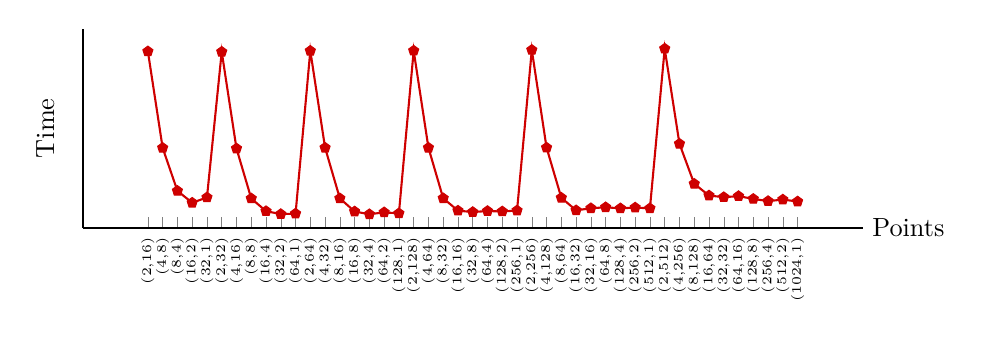
\begin{tikzpicture}[scale=.95]
\begin{axis}[
	width=0.99\textwidth,
	height=0.35\textwidth,
	xlabel=Points,
	ylabel=Time,
	axis x line*=bottom,
	axis y line*=left,
	ytick style={draw=none},
	ymin = 10.2441604675,
	ymax = 110.0,
	xticklabels={\tiny {(2,16)},\tiny {(4,8)},\tiny {(8,4)},\tiny {(16,2)},\tiny {(32,1)},\tiny {(2,32)},\tiny {(4,16)},\tiny {(8,8)},\tiny {(16,4)},\tiny {(32,2)},\tiny {(64,1)},\tiny {(2,64)},\tiny {(4,32)},\tiny {(8,16)},\tiny {(16,8)},\tiny {(32,4)},\tiny {(64,2)},\tiny {(128,1)},\tiny {(2,128)},\tiny {(4,64)},\tiny {(8,32)},\tiny {(16,16)},\tiny {(32,8)},\tiny {(64,4)},\tiny {(128,2)},\tiny {(256,1)},\tiny {(2,256)},\tiny {(4,128)},\tiny {(8,64)},\tiny {(16,32)},\tiny {(32,16)},\tiny {(64,8)},\tiny {(128,4)},\tiny {(256,2)},\tiny {(512,1)},\tiny {(2,512)},\tiny {(4,256)},\tiny {(8,128)},\tiny {(16,64)},\tiny {(32,32)},\tiny {(64,16)},\tiny {(128,8)},\tiny {(256,4)},\tiny {(512,2)},\tiny {(1024,1)}},
	x tick label style={rotate=90,anchor=east,font=\tiny},
	xlabel style={at={(1.0,0)},anchor=west, rotate=0},
%	legend style={at={(0.85,1.1)},anchor=west},
	xtick={1,...,45},
    yticklabels={,,},
	]
\addplot[sharp plot, color=contrast, mark=pentagon*] coordinates {
(1,98.6498967272)
(2,50.3064600091)
(3,28.7719769609)
(4,22.8400866484)
(5,25.4781615758)
(6,98.4383133784)
(7,50.0033584659)
(8,24.9785897802)
(9,18.6134573727)
(10,17.1407700962)
(11,17.3842588705)
(12,98.92697016)
(13,50.3862235731)
(14,25.0197309869)
(15,18.4497321623)
(16,17.0736007792)
(17,18.023206999)
(18,17.5152390388)
(19,98.9882621618)
(20,50.3719500932)
(21,25.0659098924)
(22,18.8619838458)
(23,18.173498346)
(24,18.6806266897)
(25,18.4631660258)
(26,18.9291531628)
(27,99.372806502)
(28,50.411412067)
(29,25.3194740642)
(30,19.0231902067)
(31,20.0701919363)
(32,20.557169485)
(33,20.0240130308)
(34,20.4102366039)
(35,20.0408053601)
(36,100.0)
(37,52.3610014945)
(38,32.3243942167)
(39,26.4479185908)
(40,25.6141794428)
(41,26.1490151299)
(42,24.7518933351)
(43,23.6519957683)
(44,24.4177259828)
(45,23.4639216806)
};
\addplot [mark=none, dashed]coordinates{
(1,1)
(2,1)
(3,1)
(4,1)
(5,1)
(6,1)
(7,1)
(8,1)
(9,1)
(10,1)
(11,1)
(12,1)
(13,1)
(14,1)
(15,1)
(16,1)
(17,1)
(18,1)
(19,1)
(20,1)
(21,1)
(22,1)
(23,1)
(24,1)
(25,1)
(26,1)
(27,1)
(28,1)
(29,1)
(30,1)
(31,1)
(32,1)
(33,1)
(34,1)
(35,1)
(36,1)
(37,1)
(38,1)
(39,1)
(40,1)
(41,1)
(42,1)
(43,1)
(44,1)
(45,1)
};
%\legend{\tiny {Rational-Program (\tt{X} 1, n=8192)},\tiny {CUDA (\tt{X} 1, n=8192)}}
\end{axis}
\end{tikzpicture}
\caption{Example\:polybench\\\_2DCONV\,\ Kernel\:Convolution2D\_kernel for input size 8192} \label{fig:Convolution2D_kernel-8192}
\end{figure}

    \end{block}
\end{frame}
%%%%%%%%%%%%%%%%%%%%%%%%%%%%%%%%%%%%%%%%%%%%%%%
%%%%%%%%%%%%%%%%%%%%%%%%%%%%%%%%%%%%%%%%%%%%%%%
\section{Background}
\subsection{CUDA}

\begin{frame}
    \begin{block}{Compute Unified Device Architecture}
        \begin{itemize}
            \item CUDA is a parallel programming model developed by NVIDIA, which allows developers 
            to leverage the power of GPUs for general-purpose computing.
            \item CUDA programs are written in C/C++ and executed on the GPU.
        \end{itemize}
        \begin{center}
            \begin{figure}[H]
                
\includegraphics[scale=0.5]{figures/Cuda.png}
            \end{figure}
        \end{center}        
    \end{block}
\end{frame}

\begin{frame}{Graphics Processing Units (GPUs)}
	\begin{block}{}
		\begin{itemize}
			\item GPUs are designed for massive parallelism, while CPUs focus on sequential processing.
            \item GPUs are designed to handle massive amounts of data and perform the same operation on them simultaneously.
		\end{itemize}
        \begin{center}
            \begin{figure}[H]
                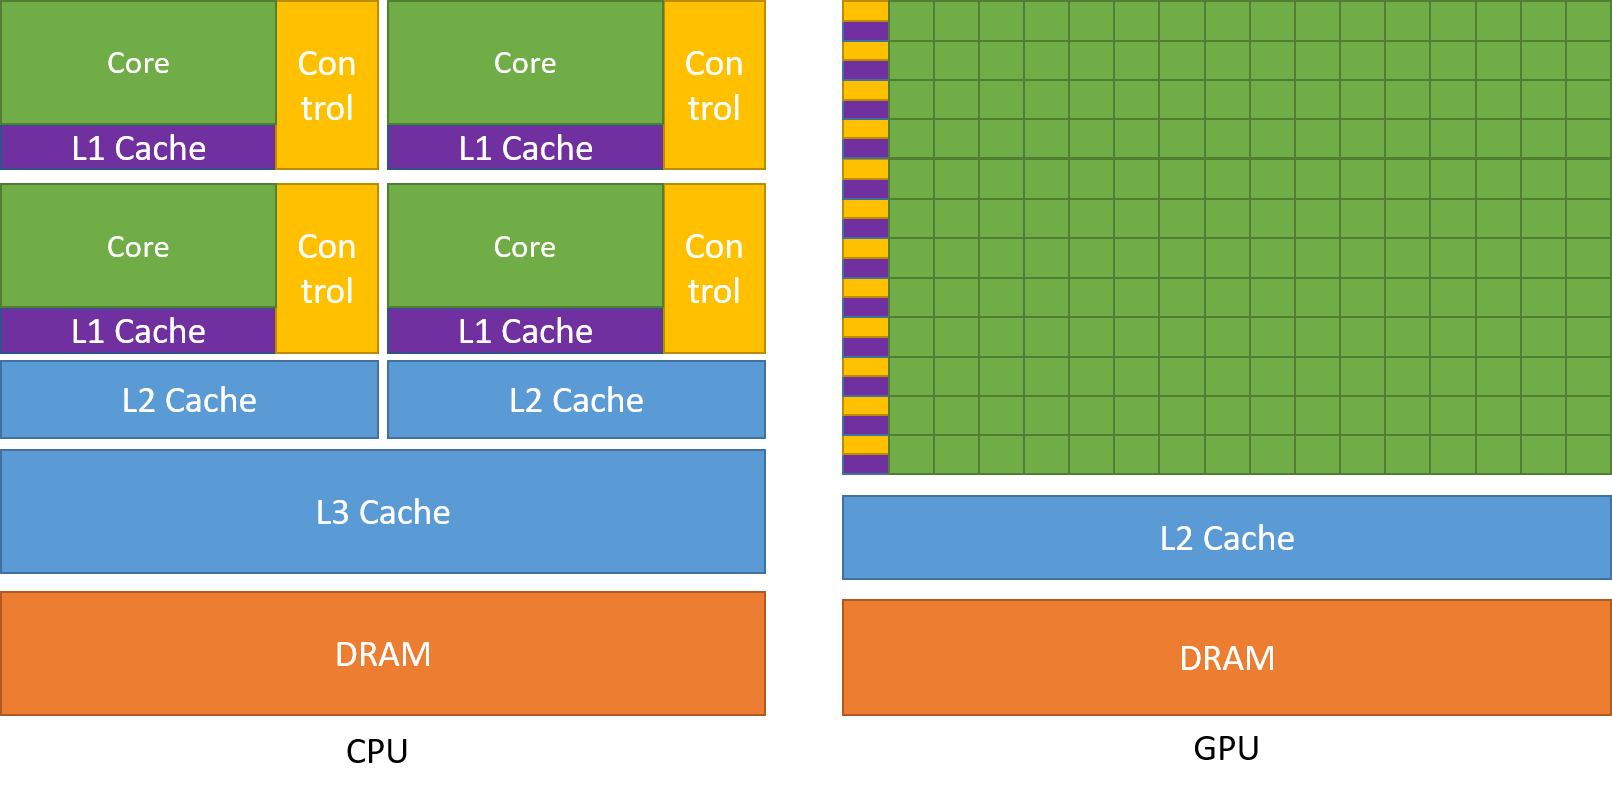
\includegraphics[scale=0.3]{figures/gpu-devotes-more-transistors-to-data-processing.png}
            \end{figure}
        \end{center}
	\end{block}
\end{frame}

\begin{frame}{GPU Microarchitecture}
    \begin{block}{}
        \begin{itemize}
            \item Streaming Multiprocessor (SM): An SM is a processing unit in a GPU that executes multiple threads concurrently. 
            It contains ALUs, registers, and shared memory, and is essential for parallel computations.
            \item Warp: A warp is a group of threads (typically 32) in a GPU that are executed simultaneously using SIMD. 
            All threads in a warp perform the same instruction on different data elements, maximizing throughput.
            \item SIMD (Single Instruction, Multiple Data): SIMD is a computing paradigm where one instruction is applied to multiple data elements concurrently. 
            GPUs use SIMD in warps for efficient parallel execution.
        \end{itemize}
        \begin{center}
            \begin{figure}[H]
                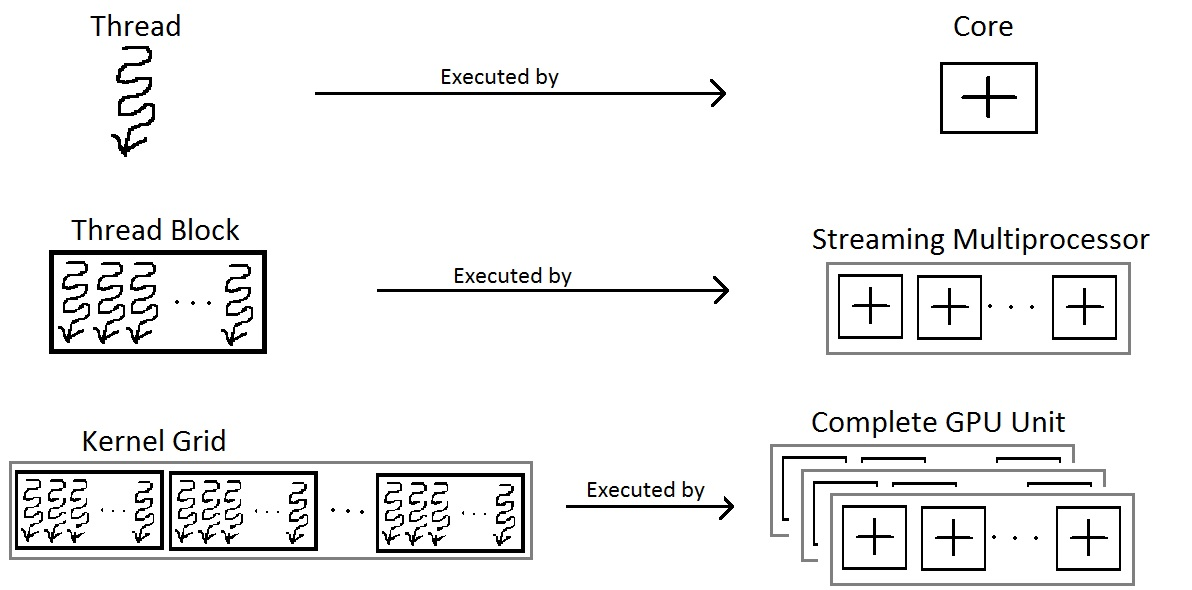
\includegraphics[scale=0.35]{figures/Software-Perspective_for_thread_block.jpg}
            \end{figure}
        \end{center}
    \end{block}
\end{frame}

\begin{frame}{CUDA Programming Model}
    \begin{block}{}
        \begin{itemize}
            \item Kernels
            \item Threads
            \item Kernel Launch Parameters
        \end{itemize}
        \begin{center}
            \begin{figure}[H]
                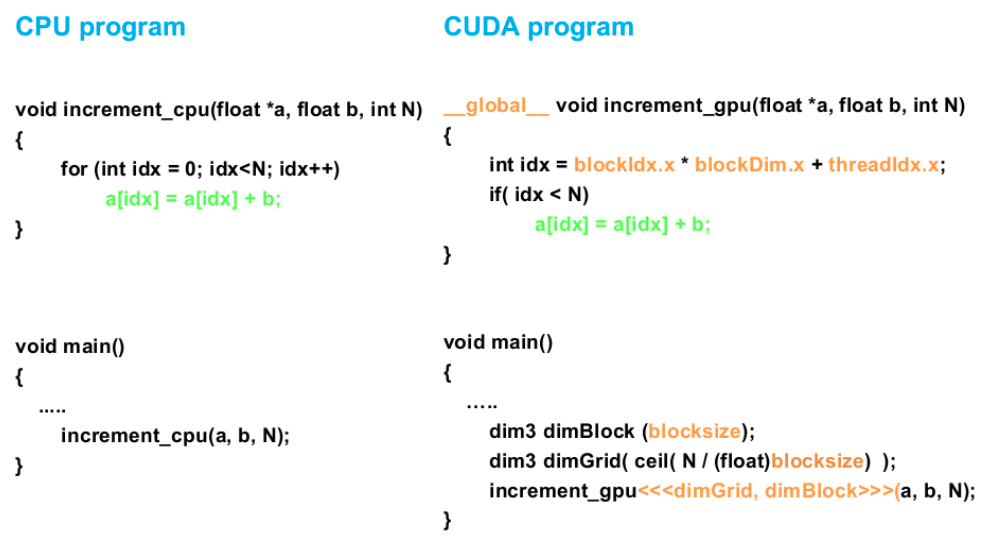
\includegraphics[scale=0.3]{figures/CPUvsGPUprogram.png}
            \end{figure}
        \end{center}
    \end{block}
\end{frame}

\begin{frame}[fragile]{Kernels}
	\begin{block}{}
        \begin{minted}{c}
// Kernel definition
__global__ void VecAdd(float* A, float* B, float* C)
{
    int i = threadIdx.x;
    C[i] = A[i] + B[i];
}

int main()
{
    ...
    // Kernel invocation with N threads
    VecAdd<<<1, N>>>(A, B, C);
    ...
}
        \end{minted}
    \end{block}            
\end{frame}

\begin{frame}{Thread Hiearchy}
	\begin{block}{}
        \begin{itemize}
            \item Threads constitute the basic units of parallel execution and 
            are organized within a hierarchical structure encompassing threads, thread blocks, and grids.
            \item Blocks can be executed in any order, both concurrently and sequentially, across the available 
            SMs on a GPU.
        \end{itemize}
        \begin{center}
            \begin{figure}[H]
                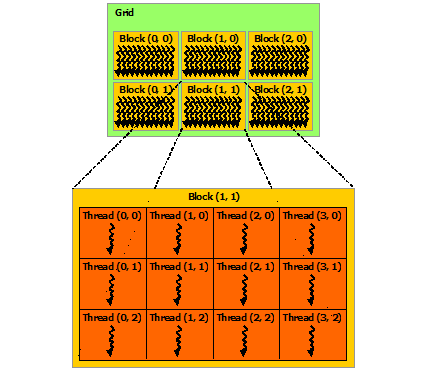
\includegraphics[scale=0.65]{figures/grid-of-thread-blocks.png}
            \end{figure}
        \end{center}
    \end{block}
\end{frame}

\begin{frame}[fragile]{Kernel Launch Parameters}
	\begin{block}{}
        \begin{itemize}
            \item Kernel launch parameters define the organization of threads and blocks for a particular kernel invocation.
            \item Optimal kernel launch parameters can significantly improve the performance of a GPU program.
            \item Finding the best kernel launch parameters is not straightforward, as they depend on the data, 
            hardware, and program characteristics.
        \end{itemize}
        \begin{minted}{c}
    //a CUDA kernel for vector addition
    __global__ void vector_addition(int *A, int *B, size_t n) {
        A[threadIdx.x] += B[threadIdx.x];
    }
    int main(){
        ...
        //launch the kernel with 1 block and n threads per block
        vector_addition<<<1, n>>>(Ad, Bd, n);
        ...
    }			
        \end{minted}
	\end{block}
\end{frame}

\begin{frame}{Heterogeneous Programming Mode}
    \begin{center}
        \begin{figure}[H]
            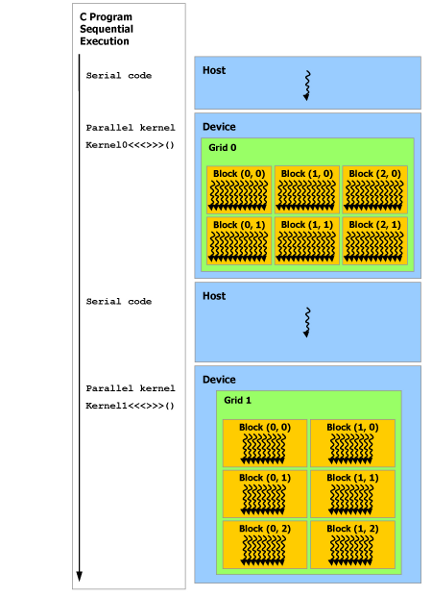
\includegraphics[scale=0.5]{figures/heterogeneous-programming.png}
        \end{figure}
    \end{center}
\end{frame}

\begin{frame}{CUDA Memory Model}
    \begin{center}
        \begin{figure}[H]
            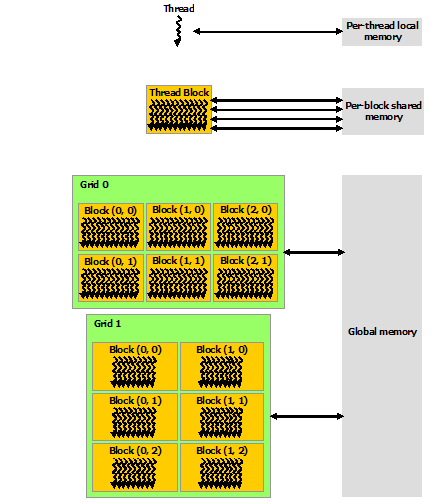
\includegraphics[scale=0.55]{figures/memory-hierarchy.png}
        \end{figure}
    \end{center}
\end{frame}

\subsection{MWP-CWP}
\begin{frame}[fragile]{Main observation of MWP-CWP}
	\begin{block}{}
        As we know, memory accesses can be overlapped between warps.
        \begin{center}
            \begin{figure}[H]
                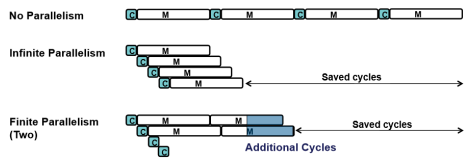
\includegraphics[scale=0.6]{figures/mwp_cwp.png}
            \end{figure}
        \end{center}
        Performance can be predicted by knowing the amount of memory-level parallelism.
    \end{block}
\end{frame}

\begin{frame}[fragile]{Memory Warp Parallelism (MWP)}
	\begin{block}{}
        MWP is the maximum number of warps that can overlap memory accesses.
        \begin{center}
            \begin{figure}[H]
                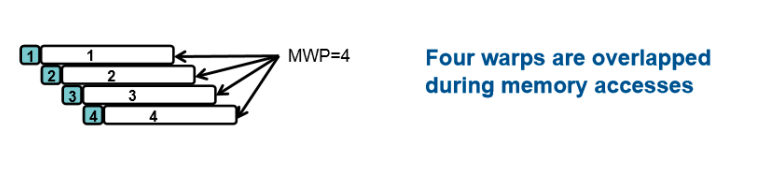
\includegraphics[scale=0.4]{figures/MWP.png}
            \end{figure}
        \end{center}
        \begin{itemize}
            \item MWP = 4.
            \item MWP is determined by \#Active SMs, \#Active warps, Bandwidth, Types of memory accesses (Coalesced, Uncoalesced)
        \end{itemize}
    \end{block}
\end{frame}

\begin{frame}[fragile]{Computation Warp Parallelism (CWP)}
	\begin{block}{}
        CWP is the number of warps that execute instructions during one memory access period plus one.
        \begin{center}
            \begin{figure}[H]
                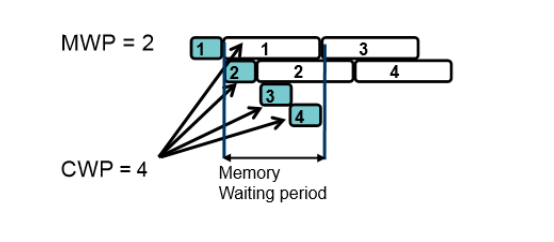
\includegraphics[scale=0.5]{figures/CWP.png}
            \end{figure}
        \end{center}
        \begin{itemize}
            \item CWP = 4.
        \end{itemize}
    \end{block}
\end{frame}

\begin{frame}{$MWP \leq CWP$}
	\begin{block}{}
        \begin{center}
            \begin{figure}[H]
                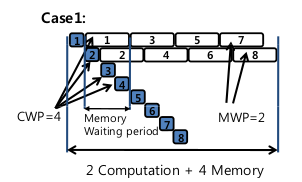
\includegraphics[scale=0.65]{figures/cwpgreater.png}
            \end{figure}
        \end{center}
        \begin{itemize}
            \item Computation cycles are hidden by memory waiting periods
            \item Overall performance is dominated by the memory cycles
        \end{itemize}
    \end{block}
\end{frame}

\begin{frame}{$MWP > CWP$}
	\begin{block}{}
        \begin{center}
            \begin{figure}[H]
                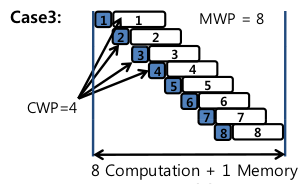
\includegraphics[scale=0.65]{figures/mwpgreater.png}
            \end{figure}
        \end{center}
        \begin{itemize}
            \item Memory accesses are mostly hidden due to high MWP
            \item Overall performance is dominated by the computation cycles
        \end{itemize}
    \end{block}
\end{frame}

\begin{frame}{Questions to answer}
	\begin{block}{}
		\begin{itemize}
			\item For a CUDA program, can we automatically and dynamically finds the values of kernel launch parameters which optimize the performance for each kernel invocation independently?
		\end{itemize}
	\end{block}
\end{frame}


%%%%%%%%%%%%%%%%%%%%%%%%%%%%%%%%%%%%%%%%%%%%%%%
%%%%%%%%%%%%%%%%%%%%%%%%%%%%%%%%%%%%%%%%%%%%%%%

\chapter{An Overview of KLARAPTOR}
\label{ch:overview}

In this chapter, we present an overview of KLARAPTOR, a compile-time tool designed to optimize the performance of 
CUDA kernels by dynamically choosing the most suitable thread block configuration. We discuss the underlying theory 
of rational programs and the MWP-CWP performance model, which form the basis of KLARAPTOR's functionality. Furthermore, 
we explain the process of building and utilizing rational programs to determine optimal kernel launch parameters, 
detailing both the compile-time and runtime aspects of the tool. This chapter aims to provide an in-depth understanding of 
KLARAPTOR's methodology and how it contributes to enhancing kernel performance in CUDA applications.

\section{Dynamic Optimization of CUDA Kernel Launch Parameters}
\label{sec:klaraptor}

%\begin{figure*}[ht]
%	\centering
%	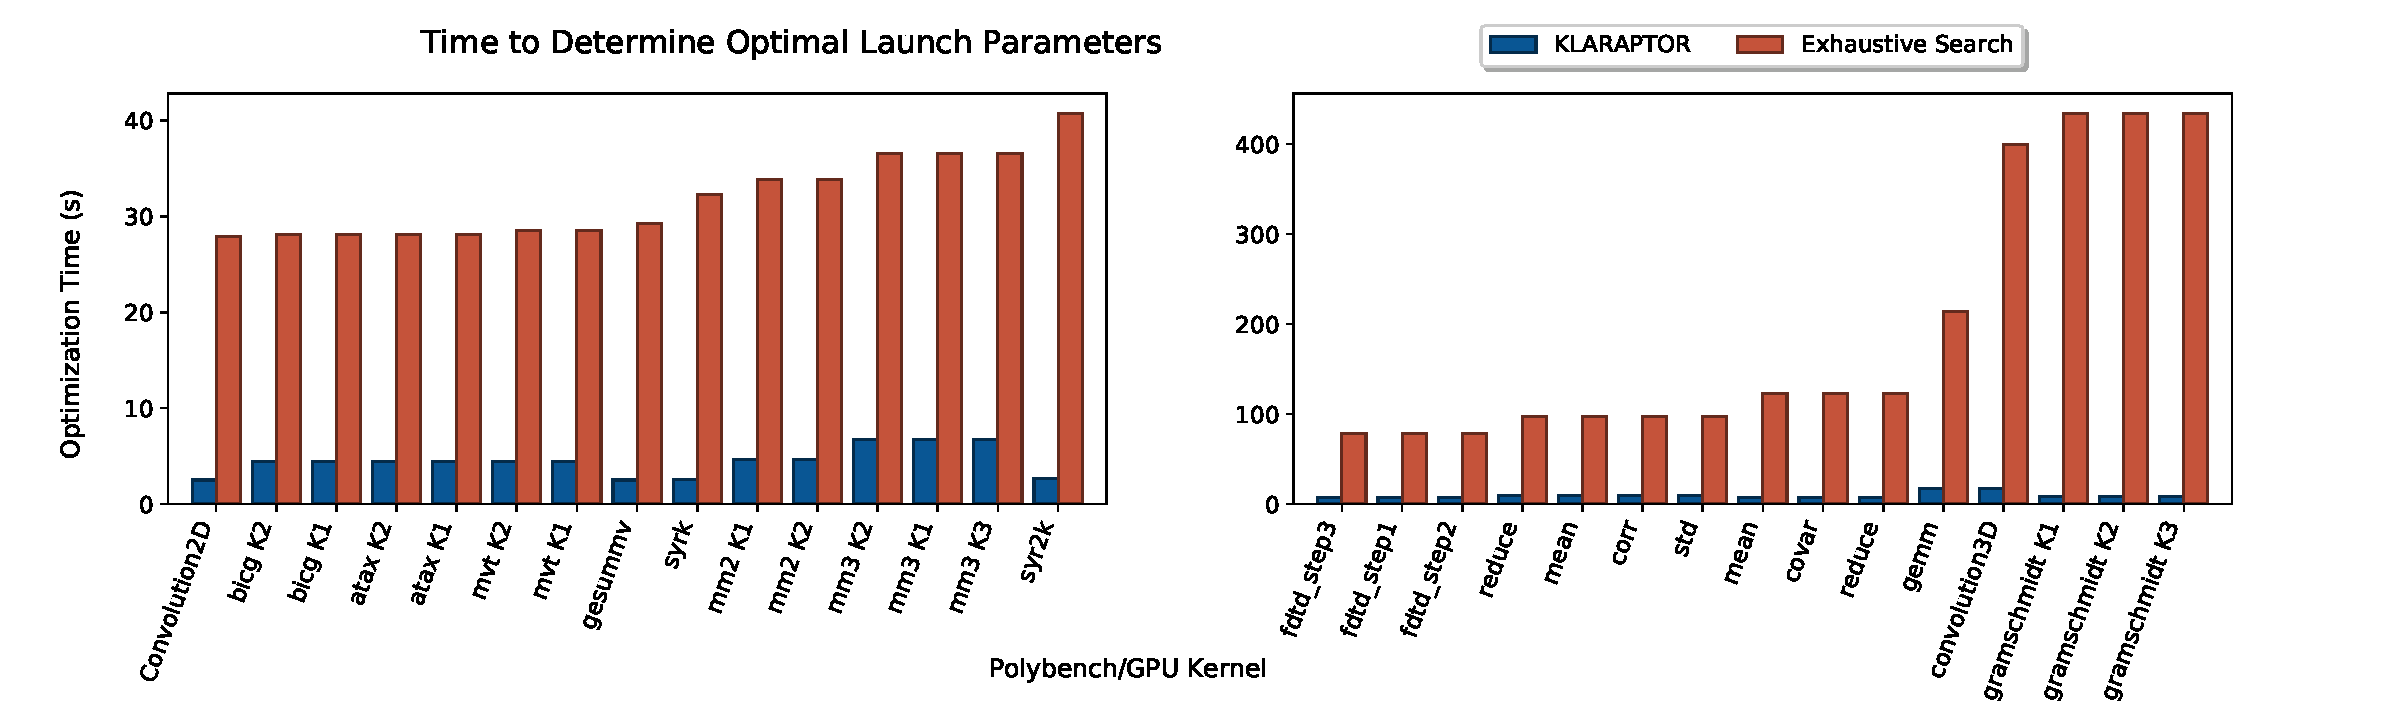
\includegraphics[width=\textwidth,clip,trim={1.5em, 1em, 5.5em, 1.2em}]{Figures/SystemTimesAll.pdf}
%	\caption{Comparing cumulative times to determine optimal launch parameters for data sizes $32 \leq N \leq 2048$ for each kernel in \texttt{Polybench/GPU}.}\label{fig:systemtimesall}
%\end{figure*}

The theory of rational programs is put into practice for the {\cuda}
programming model by our tool KLARAPTOR.  KLARAPTOR is a compile-time
tool implemented using the LLVM Pass Framework and the {\mwpcwp}
performance model to dynamically choose a {\cuda} kernel's launch
parameters (thread block configuration) which optimize its
performance.  Most high-performance computing applications require
computations be as fast as possible and so kernel performance is
simply measured as its execution time.

As mentioned in Chapter~\ref{ch:intro}, 
thread block configurations drastically affect the running time of a kernel.
Determining optimal thread block configurations typically follows some heuristics, for example, 
constraining block size to be a multiple of 32 \cite{cuda2016best}. However, it is known
that the dimension sizes of a thread block, not only its total size, affect performance~\cite{DBLP:journals/tjs/TorresGL13,DBLP:conf/cascon/ChenCKMX15}.
Moreover, since thread block configurations are intimately tied to the size of data being operated on,
it is very unlikely that a static thread block configuration optimizes the performance 
of all data sizes. Our tool effectively uses rational programs to 
dynamically determine the thread block configuration 
which minimizes the execution time of a particular 
kernel invocation, considering
the invocation's particular data size 
and target architecture. 
This is achieved in two main steps. 
\begin{enumerate}
	\item At the compile-time of a {\cuda} program, its kernels are analyzed in order to
	build rational programs estimating some performance metrics for each individual kernel.
	Each rational program, written as code in the C language,
	is inserted into the code of the {\cuda} program
	so that it is called before the execution of the corresponding kernel.
	\item At runtime, immediately preceding the launch of a kernel, where data parameters have specific values, the rational program is evaluated to 
	determine the thread block configuration which optimizes the performance of the kernel. The kernel
	is then launched using this thread block configuration. 
\end{enumerate} 

Not only are we concerned with kernel performance, but also
programmer performance. By that, 
we mean the efficiency of a programmer to produce 
optimal code. When a programmer is attempting to optimize a kernel, choosing optimal launch
parameters can either be completely ignored, 
performed heuristically, determined by trial and error, or determined by an exhaustive search.
The latter two options quickly become infeasible as data sizes grow large.
Regardless, any choice of optimal thread block configuration is likely to optimize
only a single data size. 

For KLARAPTOR to be practical, not only does the choice of optimal
kernel launch parameters need to be correct, but it must also
be more efficient than trial and error or exhaustive search.
Namely, the compile-time analysis cannot add too much 
overhead to the the compilation time and the
runtime decision of the kernel launch parameters cannot
overwhelm the program execution time. 
For the former, our analysis is performed
quickly by analyzing kernel performance on only small data sizes, 
and then results are extrapolated.
For the later, the rational program evaluation is quick and simple, 
being only the evaluation of a few rational functions.
Moreover, we maintain a runtime invocation history
to instantly provide results for future kernel launches.
Our implementation is detailed in Chapter~\ref{ch:implementation}.
%In the remainder of this section we highlight the performance of
%KLARAPTOR.

We have made use of the \texttt{Polybench/GPU}
benchmark suite as an empirical
evaluation of the correctness of our tool on a range of {\cuda} programs.
In Figure~\ref{fig:kernelperfintro} we have already seen that KLARAPTOR
accurately predicts the optimal or near-optimal thread block
configuration. 
Before presenting more detailed results and 
experimentation in Chapter~\ref{ch:performance},
we describe the steps followed by our tool
to build and use rational programs for 
determining a thread block configuration which optimizes
performance.

%Let us begin with kernel performance. 
%Other optimization techniques (see Section~\ref{sec:relatedworks})
%focus on improving the performance of a kernel by code optimizations. Our techniques
%rather focuses on simply modifying program parameters for performance. 
%focus on auto-tuning, static source code analysis, or machine learning applied to over-simplified 
%models.


\section{An Algorithm to Select Program Parameters}
\label{sec:steps}

In this section the notations and hypotheses are the same as in
Chapter~\ref{ch:foundations}.
Namely, ${\cal E}$ is a high-level performance metric for the 
multithreaded program ${\cal P}$, 
${\bm L}$ is a set of low-level metrics of size $\ell$,
and ${\bm P}$, ${\bm D}$, ${\bm H}$ are
sets of program, data, and hardware parameters, respectively. 
Recall ${\bm P}$ has size $p$.
%%
Let us assume that the values of ${\bm H}$ are known at the compile-time of ${\cal P}$
while the values of ${\bm D}$ are known at runtime.
Further, let us assume that ${\bm P}$ and ${\bm D}$
take integer values. 
Hence the values of ${\bm P}$ belong to a finite set $F \subset \mathbb{Z}^p$.
%
%
%In particular, we assume that:
%\begin{enumerateshort}
%\item[$(i)$] ${\cal E}$
%is a high-level performance metric for the multithreaded program ${\cal P}$
%(e.g. execution time, memory
%consumption, and hardware occupancy),
%\item[$(ii)$] ${\cal E}$ is given (by a program execution model, e.g. {\cuda}
%or MWP-CWP) as a rational program depending on hardware parameters
%${\bm{H}}$, low-level performance metrics $\bm{L}$, and program parameters $\bm{P}$ (see Examples~\ref{ex:cuda} 
%and \ref{ex:mwpcwp}),
%\item[$(iii)$] the values of the hardware parameters %$H_1, \ldots, H_h$
%are known at compile-time for ${\cal P}$
%while the values of the data parameters $\bm{D}$
%are known at runtime for ${\cal P}$, 
%\item[$(iv)$] the data and program parameters 
%%$\bm{D}$, $\bm{P}$
%take integer values.
%\end{enumerateshort}
%%%
%Extending $(iv)$ we further assume that the possible values of 
%the program
%parameters $\bm{P}$ belong to a finite set $F \,\subset\, \mathbb{Z}^p$.
That is to say, the possible values of
$\bm{P}$ are tuples of the form $(\pi_1, \ldots, \pi_p) \in F$,
with each $\pi_i$ being an integer.
Let us call such a tuple a \textit{configuration} of the program parameters.
Due to the nature of program parameters, those are not necessarily all
independent variables 
%(i.e. a program parameter may depend on the value of
%another program parameter). 
%For example, in {\cuda} the product of thread block dimensions should be a power of 32.
For example, in {\cuda}, the product of the dimension sizes
of a thread block is usually
%\begin{inparaenum}[(i)]
%\item 
a multiple of the warp size (32).
%, and
%\item 
%bounded by the maximum number of threads per block.
%\end{inparaenum}

Given a performance-prediction model for ${\cal E}$, 
one could work recursively to determine a 
single helper program ${\cal R}$, depending on only
$\bm{D}$ and $\bm{P}$, evaluating ${\cal E}$,
from a combination of rational programs constructed
for each low-level metric in $\bm{L}$
and values of $\bm{D}$ and $\bm{P}$.
Following Section~\ref{sec:prf_rp}, 
each of these helper programs are constructed by 
computing rational functions. Without loss of generality,
let us assume each low-level metric is given
by a single formula and thus a single rational function. 
Hence, we look to determine $g_1(\bm{D}, \bm{P})$,
$\ldots$, $g_{\ell}(\bm{D}, \bm{P})$ for the $\ell$ 
low-level metrics.
Finally, at runtime, given particular values of $\bm{D}$,
the helper program for ${\cal E}$ can be evaluated
for various values of $\bm{P}$ to determine
the optimal configuration.
%
%However, in the context of {\cuda} we have not
%found a particularly suitable model.
%Instead, using rational functions
%for the evaluation of some low-level performance
%metrics (e.g. amount of shared memory used per thread block),
%we follow a decision tree coupled with some heuristics
%to determine the optimal configuration.
%This specialization of our general technique to {\cuda} 
%is discussed in Section~\ref{sec:heuristics}.
%
In the remainder of this section we 
describe the general process to build
and use helper programs to determine 
optimal configurations.
%%
The entire process is decomposed into five steps:
the first three occur at compile-time and the next three 
at runtime.
%Figure~\ref{fig:sixsteps} summarizes the six steps.

\begin{enumerate}
\item \textbf{Data collection}: 
%%
To perform a curve fitting of the rational functions 
$g_1(\bm{D}, \bm{P})$, $\ldots$, $g_{\ell}(\bm{D}, \bm{P})$
we require data points to fit. These are collected by 
\begin{inparaenum}[(i)]
\item selecting a subset of $K$ points
from the space of possible values of $(\bm{D}$, $\bm{P})$; and
%%
\item executing the program ${\cal P}$, recording the values of
       the low-level performance metrics $\bm{L}$ as
       ${\bm V} = (V_1, \ldots, V_{\ell})$, at each point in $K$.
\end{inparaenum}
\fixed{The data used for executing the programs is generated randomly,
but could follow some scheme provided by the user.}{Is this correct?
Davood: Totally correct.}
%%
%%
\item \textbf{Rational function approximation}: 
%%
For each low-level metric $L_i$ we use the set of points $K$ 
and the corresponding value $V_i$ measured at each point
in order to approximate
the rational function $g_i(\bm{D},\bm{P})$.
\iflongversion
We observe that if these values
were known exactly the rational function
$g_i(\bm{D}, \bm{P})$ could be determined exactly.
In practice, however, these
\else
In practice, these
\fi
empirical values are likely to be noisy from profiling,
and/or numerical approximations.
%Hence, techniques from numerical analysis, like the method of least squares,
%must be used instead. 
Consequently, we actually determine a rational function
$\hat{g}_i(\bm{D}, \bm{P})$ which approximates
$g_i(\bm{D}, \bm{P})$.
%when evaluated at the points $K_1, \ldots, K_k$.
%%
%%
\item \textbf{Code generation}: 
%%
In order to generate the helper program ${\cal R}$, we 
proceed as follows:
\begin{enumerateshort}
\item[(i)] we convert the helper program representing 
${\cal E}$ into code, 
%say in the C programming language, 
%essentially encoding the flowchart for computing $\cal{E}$;
%%
\item[(ii)] we convert each
$\hat{g}_i(\bm{D}, \bm{P})$
into a sub-routine estimating $L_i$, and
%%
\item[(iii)] we include those sub-routines
into the code computing ${\cal E}$, which yields
the desired helper program ${\cal R}$ depending only on $\bm{D}$ and $\bm{P}$.
%%
\end{enumerateshort}
%At this point the rational program ${\cal R}$ is fully determined.
%%
%%
\item \textbf{Helper program evaluation}: 
%%
At the runtime of ${\cal P}$, the data parameters $\bm{D}$ are given
particular values.
% say ${\delta}_1, \ldots, {\delta}_d$.
For those specified values of $\bm{D}$ and for
all practically meaningful values of $\bm{P}$ from
the set $F$,\footnote{The values for
$\bm{P}$ are likely to be constrained by
the values $\bm{D}$.  For example,
if $P_1, P_2$ are the two dimension sizes of a two-dimensional
thread block of a {\cuda} kernel operating on a
square matrix of order $D_1$, then $P_1 P_2 \leq D_1^2$
is meaningful.} we compute an estimate of ${\cal E}$ using ${\cal R}$.
The evaluation of ${\cal E}$ over so many different possible
program parameters is feasible for three reasons:
\begin{enumerateshort}
\item[(i)] the number of program parameters is small, typically $p \leq 3$,
      see Chapter~\ref{ch:implementation};
\item[(ii)]  the set of meaningful values for ${\bm P}$ is small
	(consider that in {\cuda} the product of thread block dimension sizes should be a multiple of 32 less than 1024), and 
\item[(iii)]  the program ${\cal R}$ simply evaluates 
       a few polynomial formulae and thus runs almost instantaneously.
\end{enumerateshort}
%%
%%
\item \textbf{Program execution}: 
%
Once an optimal configuration is selected, the
program ${\cal P}$ is  executed using this
configuration along with the values
% ${\delta}_1, \ldots, {\delta}_d$
of $\bm{D}$.

%%
\end{enumerate}



\section{Implementation of KLARAPTOR}

\begin{frame}[fragile]{Annotations and preprocessing source code}
    \begin{block}{}
        \begin{minted}{c}
        
#pragma kernel_info_size_param_idx_Sample = 1; 
#pragma kernel_info_dim_sample_kernel = 2;

__global__ void Sample (int *A, int N) { 
    int tid_x = threadIdx.x + blockIdx.x*blockDim.x;
    int tid_y = threadIdx.y + blockIdx.y*blockDim.y;
    ...
}
        \end{minted}
        \begin{itemize}
            \item Annotating and preprocessing the source code makes it compatible with the KLARAPTOR tool, 
            enabling the automatic determination of optimal kernel launch parameters.
            \item CUDA program should target at least CUDA Compute Capability 7.5, no CUDA runtime API calls, 
            and block and grid dimensions must be declared as dim3 structs.
            \item Add two pragmas for each kernel, specifying kernel dimension and the 
            index of the kernel input argument corresponding to the data size N
        \end{itemize}
    \end{block} 
\end{frame}

\begin{frame}{Input/Output builder}
    \begin{block}{}
        The Input/Output Builder Pass creates an "instrumented binary" that embeds an IO mechanism to communicate with the 
        helper program for each kernel invocation, obtaining optimal kernel launch parameters at runtime.
        \begin{itemize}
            \item (i) Obtain the LLVM intermediate representation (IR) of the instrumented source code and find all CUDA driver 
            API kernel calls.
            \item (ii) Using the annotated information for each kernel, determine which variables in the IR contain the value 
            of N for a corresponding kernel call.
            \item (iii) Insert a call to an IO function immediately before each kernel call to pass the runtime value of N to 
            the corresponding helper program and retrieve the optimal kernel launch parameters.
        \end{itemize}
    \end{block}
\end{frame}

\begin{frame}{Building a helper program: data collection}
    \begin{block}{}
        Data collection is necessary to perform rational function approximation and gather metrics on performance 
        counters and runtime metrics.
        \begin{itemize}
            \item (i) Architecture-specific performance counters influenced by the Compute Capability (CC) of the device.
            \item (ii) Runtime-specific performance counters that depend on the kernel's behavior, including memory access 
            patterns and the number of executed warps.
            \item (iii) Device-specific parameters describing the actual GPU card, including memory bandwidth, departure delay for 
            memory accesses, number of SMs, clock frequency, and instruction delay.
        \end{itemize}
    \end{block}
\end{frame}

\begin{frame}[fragile]{Building a helper program: data collection}
    \begin{block}{Runtime-specific performance counters}
        {
            \begin{tcolorbox}
                \scriptsize
                \begin{verbatim}
[trace: n=4096, bx=32, by=8, elapsed_Convolution2D_kernel=219.9013 (ms)] ... PASS
==PROF== Disconnected from process 41150
"Metric Name","Metric Unit","Metric Value"
"dram__bytes_read.sum","byte","68,456,288"
"dram__bytes_write.sum","byte","66,864,032"
"l1tex__t_bytes_pipe_lsu_mem_global_op_ld.sum.per_second","byte/second","1,293,146,285,512.62"
"l1tex__t_bytes_pipe_lsu_mem_global_op_st.sum.per_second","byte/second","123,294,394,447.39"
"l1tex__t_sectors_pipe_lsu_mem_global_op_ld.sum","sector","21,984,780"
"l1tex__t_sectors_pipe_lsu_mem_global_op_st.sum","sector","2,096,128"
"launch__block_dim_x","block","32"
"launch__block_dim_y","block","8"
"launch__block_dim_z","block","1"
"launch__grid_dim_x","","128"
"launch__grid_dim_y","","512"
"launch__grid_dim_z","","1"
"launch__registers_per_thread","register/thread","30"
"launch__shared_mem_per_block_dynamic","byte/block","0"
"launch__shared_mem_per_block_static","byte/block","0"
"sm__warps_active.avg.pct_of_peak_sustained_active","%","87.46"
"smsp__average_inst_executed_per_warp.ratio","inst/warp","46.98"
"smsp__inst_executed.avg.per_cycle_active","inst/cycle","0.18"
"smsp__inst_executed_op_global_ld.sum","inst","4,716,288"
"smsp__inst_executed_op_global_st.sum","inst","524,032"
\end{verbatim}
\end{tcolorbox}
        }
    \end{block}
\end{frame}

\begin{frame}[fragile]{Building a helper program: data collection}
    \begin{block}{Device-specific parameters}
        {
            \begin{tcolorbox}
                \scriptsize
                \begin{verbatim}
[Issue_cycles: 1]
[Mem_bandwidth: 448.06]
[Mem_LD: 501]
[Departure_del_uncoal: 2]
[Departure_del_coal: 2]
[Active_SMs: 40]
[Freq: 1785]
[Load_bytes_per_warp: 128]

[device_name: NVIDIA GeForce RTX 2070 SUPER]
[driver_version: 11.7]
[runtim_version: 11.7]
[compute_capability: 7.5]
[global_memory_bytes: 8361803776]
[n_cores_per_sm:  64]
[n_blocks_per_sm: 32]
[n_cores: 2560]
[memory_clock_rate_ghz: 7.00]
[memory_bus_width_bits: 256]
[l2_cache_size_bytes: 4194304]
[total_constant memory_bytes: 65536]
[total_shared_memory_per_block_bytes: 49152]
[total_registers_available_per_block: 65536]
[warp_size: 32]
                \end{verbatim}
            \end{tcolorbox}
        }           
    \end{block}
\end{frame}

\begin{frame}[fragile]{Building a helper program: outlier removal}
    \begin{block}{}
        \begin{itemize}
            \item Outlier removal addresses potential noise in the empirical data gathered from NVIDIA’s Nsight Compute 
            (ncu) and enhances the accuracy of the parameter estimation process.
            \begin{itemize}
                \item (i) Profile the program for small input sizes and obtain MWP-CWP estimation for clock-cycles 
                for various thread block configurations.
                \item (ii) Calculate Q1, Q3, and IQR for the estimated clock-cycles and determine the upper inner fence.
                \item (iii) Identify and remove outliers exceeding the upper inner fence threshold.
            \end{itemize}
        \end{itemize}
        {
            \begin{tcolorbox}
                \scriptsize
                \begin{verbatim}
128 1 32 72869.600000
128 1 64 78474.600000
128 1 128 89684.600000
256 1 64 294064.600000
256 1 32 361929.200000
512 1 32 1271232.200000
512 1 64 1452818.400000
1024 1 64 4729979.800000
1024 1 32 4730039.600000
2048 1 32 18771193.800000
2048 1 64 18953199.200000
2048 1 512 18953199.200000
2048 1 1024 18953199.200000
                \end{verbatim}
            \end{tcolorbox}
        }
    \end{block}
\end{frame}

\begin{frame}[fragile]{Building a helper program: rational function approximation}
    \begin{block}{}
        \begin{itemize}
            \item The goal of this step is to determine rational functions that estimate low-level performance metrics or other intermediate values in the rational program ${\cal R}$. These rational functions are used to build the objective function ${\cal E} = f({\bm P}, {\bm D}, {\bm H})$
            \item A rational function is a fraction of two polynomials, with defined degree bounds on each variable, 
            the polynomials can be represented by coefficients that we aim to estimate: 
            {
                \small
                    \begin{align}
                    f(X_1,\dots,X_n) &= \frac{\alpha_1\cdot(X_1^0\cdots X_n^0) \;+\; 
                        \dots \;+\;  \alpha_i\cdot(X_1^{u_1}\cdots X_n^{u_n})}{\beta_1\cdot(X_1^0\cdots X_n^0) \;+\;
                        \dots \;+\; \beta_j\cdot(X_1^{v_1}\cdots X_n^{v_n})}
                    \end{align}
            }
            \item We perform parameter estimation on the coefficients of the polynomials in the rational function. 
            The estimation process involves solving an over-determined system of linear equations.
            \item We use numerical analysis techniques such as singular value decomposition (SVD) and linear least squares 
            to solve the system.
        \end{itemize}
    \end{block}
\end{frame}
\section{Experimentation}

\begin{frame}[fragile]{}
    \begin{figure}[t!]
        \includegraphics[width=\textwidth, trim={0em, 0.9em, 0em, 0em}, clip]{figures/MinMaxTimes-RTX-8192.png}
        \caption{Comparing kernel execution time (log-scaled) for the thread block configuration chosen by KLARAPTOR
            versus the minimum and maximum times as determined by an exhaustive search over all possible configurations. 
            Kernels are part of the \texttt{PolyBench/GPU} benchmark suite and executed on a RTX 2070 SUPER with a data 
            size of $N=8192$ (except convolution3d with $N=512$)}
    \end{figure}
\end{frame}

\begin{frame}[fragile]{}
    \begin{table}[htb]
    \centering
    \scriptsize
    \caption{KLARAPTOR Optimization Times on \texttt{Polybench/GPU}, RTX 2070 SUPER
    Comparing times for (1) compile-time optimization steps of KLARAPTOR, (2) exhaustive search over all 
    thread block configurations, the execution time for a kernel given (3) the best thread block configuration, and (4) 
    the worst thread block configuration. Exhaustive search is given as a sum for values up to $N=8192$ (except convolution3d with $N=512$).}\label{table:opttimetable}
    \setlength{\tabcolsep}{0.6em}
    \renewcommand{\arraystretch}{1.25}
    \begin{tabular}{l|rr|rr}
        \toprule
        Kernel &  KLARAPTOR Time (s) &  Ex. Search Time (s) &  Min Time (s) &  Max Time (s) \\
        & $128 \leq N<\infty$ & $128 \leq N \leq 8192$ & $N=8192$ & $N=8192$\\
        \midrule
            2DCONV &              210.29 &                       82.78 &      0.002 &         0.023 \\
            ATAX &              507.59 &                       59.60 &        0.006 &         1.940 \\
                MVT &              508.03 &                       60.03 &     0.005 &         1.978 \\
            BICG &              510.91 &                       60.16 &        0.006 &         2.050 \\
            GESUMMV &              398.54 &                      142.78 &     0.006 &         0.129 \\
            GEMM &              456.50 &                      987.77 &        3.941 &       126.052 \\
            SYRK &              579.84 &                     2772.64 &        9.069 &       160.944 \\
            SYR2K &             1173.68 &                     9553.64 &       15.534 &       459.169 \\
                2MM &              700.49 &                     1889.62 &     7.851 &       240.828 \\
                3MM &              944.54 &                     2798.12 &     11.779 &       361.310 \\
            CORR &             1032.92 &                    10924.12 &        28.365 &       861.289 \\
            COVAR &             1141.45 &                    23251.12 &       27.670 &      3900.855 \\
            3DCONV &              132.88 &                       52.06 &      0.006 &         0.053 \\
        GRAMSCHM &             2113.27 &                    94206.06 &        45.418 &     35146.314 \\
            FDTD\_2D &              489.21 &                      495.79 &     3.304 &        21.107 \\
        \bottomrule
    \end{tabular}
\end{table}
\end{frame}

\section{Summary}
\begin{frame}{Summary}
	\textbf{KLARAPTOR: A Tool for Dynamically Finding Optimal Kernel
		Launch Parameters Targeting CUDA Programs}
	\begin{itemize}
	\item We present KLARAPTOR, a freely available tool built on top
	of the LLVM Pass Framework and NVIDIA Nsight Comute CLI to dynamically determine the optimal values of kernel launch parameters of
	a CUDA kernel. 
	\item We describe a technique to build at the compile-time of a CUDA program a so-called helper program. The helper
	program, based on some performance prediction model, and knowing particular data and hardware parameters at runtime, can be
	executed to automatically and dynamically determine the values
	of launch parameters for the CUDA program. 
	\item Our underlying technique could be applied to
	parallel programs in general, given a performance prediction model
	which accounts for program and hardware parameters. 
	\item We have implemented and successfully tested our technique in the context
	of GPU kernels written in CUDA.
\end{itemize}
\end{frame}

\begin{frame}{Future work}
	\begin{block}{KLARAPTOR}
		\begin{itemize}
			\item Investigate the complexity of efficiently utilizing available hardware resources in GPU execution.
			\item Reevaluate the use of linear least squares for extrapolation beyond the "training" range.
            \item Test the model with multiples of 32 within the training range to more accurately capture CUDA thread block dimensions.
            \item Investigate random forest regression as an alternative approach, given the tree-like structure of rational programs.
            \item Explore the potential of machine learning models, such as neural networks, for determining optimal thread block configurations.
		\end{itemize}
	\end{block}
\end{frame}
\newcounter{finalframe}
\setcounter{finalframe}{\value{framenumber}}


\begin{frame}[noframenumbering,plain]
\begin{center}
	{\huge{\textbf{Thank You!}}}
\end{center}
\end{frame}
%%####################
\begin{frame}[noframenumbering,plain]
\begin{center}
{\huge{\textbf {Your Questions?}}}
\end{center}
\end{frame}
%%%####################
\bibliographystyle{abbrv} % (change according to your preference)
%%% ***   Set the bibliography file.   ***
%\bibliography{../reference}{}
%%% ***   Set the bibliography file.   ***
\bibliography{westernthesis}{}

%\begin{frame}[noframenumbering,plain]
%\begin{center}
%	{\huge{\textbf {Appendix}}}
%\end{center}
%\end{frame}

%\include{Chapters/Appendix}
%\setcounter{framenumber}{\value{finalframe}}

\end{document}
